
% Default to the notebook output style

    


% Inherit from the specified cell style.




    
\documentclass[11pt]{article}

    \usepackage[spanish]{babel}
    \usepackage{tocloft}
    \usepackage{fancyhdr}
    \usepackage{parskip}
    \usepackage{indentfirst} 
    
    
    \usepackage[T1]{fontenc}
    % Nicer default font than Computer Modern for most use cases
    \usepackage{palatino}

    % Basic figure setup, for now with no caption control since it's done
    % automatically by Pandoc (which extracts ![](path) syntax from Markdown).
    \usepackage{graphicx}
    % We will generate all images so they have a width \maxwidth. This means
    % that they will get their normal width if they fit onto the page, but
    % are scaled down if they would overflow the margins.
    \makeatletter
    \def\maxwidth{\ifdim\Gin@nat@width>\linewidth\linewidth
    \else\Gin@nat@width\fi}
    \makeatother
    \let\Oldincludegraphics\includegraphics
    % Set max figure width to be 80% of text width, for now hardcoded.
    \renewcommand{\includegraphics}[1]{\Oldincludegraphics[width=.8\maxwidth]{#1}}
    % Ensure that by default, figures have no caption (until we provide a
    % proper Figure object with a Caption API and a way to capture that
    % in the conversion process - todo).
    \usepackage{caption}
    \DeclareCaptionLabelFormat{nolabel}{}
    \captionsetup{labelformat=nolabel}

    \usepackage{adjustbox} % Used to constrain images to a maximum size 
    \usepackage{xcolor} % Allow colors to be defined
    \usepackage{enumerate} % Needed for markdown enumerations to work
    \usepackage{geometry} % Used to adjust the document margins
    \usepackage{amsmath} % Equations
    \usepackage{amssymb} % Equations
    \usepackage{textcomp} % defines textquotesingle
    % Hack from http://tex.stackexchange.com/a/47451/13684:
    \AtBeginDocument{%
        \def\PYZsq{\textquotesingle}% Upright quotes in Pygmentized code
    }
    \usepackage{upquote} % Upright quotes for verbatim code
    \usepackage{eurosym} % defines \euro
    \usepackage[mathletters]{ucs} % Extended unicode (utf-8) support
    \usepackage[utf8x]{inputenc} % Allow utf-8 characters in the tex document
    \usepackage{fancyvrb} % verbatim replacement that allows latex
    \usepackage{grffile} % extends the file name processing of package graphics 
                         % to support a larger range 
    % The hyperref package gives us a pdf with properly built
    % internal navigation ('pdf bookmarks' for the table of contents,
    % internal cross-reference links, web links for URLs, etc.)
    \usepackage{hyperref}
    \usepackage{longtable} % longtable support required by pandoc >1.10
    \usepackage{booktabs}  % table support for pandoc > 1.12.2
    \usepackage[normalem]{ulem} % ulem is needed to support strikethroughs (\sout)
                                % normalem makes italics be italics, not underlines
    

    
    
    % Colors for the hyperref package
    \definecolor{urlcolor}{rgb}{0,.145,.698}
    \definecolor{linkcolor}{rgb}{.71,0.21,0.01}
    \definecolor{citecolor}{rgb}{.12,.54,.11}

    % ANSI colors
    \definecolor{ansi-black}{HTML}{3E424D}
    \definecolor{ansi-black-intense}{HTML}{282C36}
    \definecolor{ansi-red}{HTML}{E75C58}
    \definecolor{ansi-red-intense}{HTML}{B22B31}
    \definecolor{ansi-green}{HTML}{00A250}
    \definecolor{ansi-green-intense}{HTML}{007427}
    \definecolor{ansi-yellow}{HTML}{DDB62B}
    \definecolor{ansi-yellow-intense}{HTML}{B27D12}
    \definecolor{ansi-blue}{HTML}{208FFB}
    \definecolor{ansi-blue-intense}{HTML}{0065CA}
    \definecolor{ansi-magenta}{HTML}{D160C4}
    \definecolor{ansi-magenta-intense}{HTML}{A03196}
    \definecolor{ansi-cyan}{HTML}{60C6C8}
    \definecolor{ansi-cyan-intense}{HTML}{258F8F}
    \definecolor{ansi-white}{HTML}{C5C1B4}
    \definecolor{ansi-white-intense}{HTML}{A1A6B2}

    % commands and environments needed by pandoc snippets
    % extracted from the output of `pandoc -s`
    \providecommand{\tightlist}{%
      \setlength{\itemsep}{0pt}\setlength{\parskip}{0pt}}
    \DefineVerbatimEnvironment{Highlighting}{Verbatim}{commandchars=\\\{\}}
    % Add ',fontsize=\small' for more characters per line
    \newenvironment{Shaded}{}{}
    \newcommand{\KeywordTok}[1]{\textcolor[rgb]{0.00,0.44,0.13}{\textbf{{#1}}}}
    \newcommand{\DataTypeTok}[1]{\textcolor[rgb]{0.56,0.13,0.00}{{#1}}}
    \newcommand{\DecValTok}[1]{\textcolor[rgb]{0.25,0.63,0.44}{{#1}}}
    \newcommand{\BaseNTok}[1]{\textcolor[rgb]{0.25,0.63,0.44}{{#1}}}
    \newcommand{\FloatTok}[1]{\textcolor[rgb]{0.25,0.63,0.44}{{#1}}}
    \newcommand{\CharTok}[1]{\textcolor[rgb]{0.25,0.44,0.63}{{#1}}}
    \newcommand{\StringTok}[1]{\textcolor[rgb]{0.25,0.44,0.63}{{#1}}}
    \newcommand{\CommentTok}[1]{\textcolor[rgb]{0.38,0.63,0.69}{\textit{{#1}}}}
    \newcommand{\OtherTok}[1]{\textcolor[rgb]{0.00,0.44,0.13}{{#1}}}
    \newcommand{\AlertTok}[1]{\textcolor[rgb]{1.00,0.00,0.00}{\textbf{{#1}}}}
    \newcommand{\FunctionTok}[1]{\textcolor[rgb]{0.02,0.16,0.49}{{#1}}}
    \newcommand{\RegionMarkerTok}[1]{{#1}}
    \newcommand{\ErrorTok}[1]{\textcolor[rgb]{1.00,0.00,0.00}{\textbf{{#1}}}}
    \newcommand{\NormalTok}[1]{{#1}}
    
    % Additional commands for more recent versions of Pandoc
    \newcommand{\ConstantTok}[1]{\textcolor[rgb]{0.53,0.00,0.00}{{#1}}}
    \newcommand{\SpecialCharTok}[1]{\textcolor[rgb]{0.25,0.44,0.63}{{#1}}}
    \newcommand{\VerbatimStringTok}[1]{\textcolor[rgb]{0.25,0.44,0.63}{{#1}}}
    \newcommand{\SpecialStringTok}[1]{\textcolor[rgb]{0.73,0.40,0.53}{{#1}}}
    \newcommand{\ImportTok}[1]{{#1}}
    \newcommand{\DocumentationTok}[1]{\textcolor[rgb]{0.73,0.13,0.13}{\textit{{#1}}}}
    \newcommand{\AnnotationTok}[1]{\textcolor[rgb]{0.38,0.63,0.69}{\textbf{\textit{{#1}}}}}
    \newcommand{\CommentVarTok}[1]{\textcolor[rgb]{0.38,0.63,0.69}{\textbf{\textit{{#1}}}}}
    \newcommand{\VariableTok}[1]{\textcolor[rgb]{0.10,0.09,0.49}{{#1}}}
    \newcommand{\ControlFlowTok}[1]{\textcolor[rgb]{0.00,0.44,0.13}{\textbf{{#1}}}}
    \newcommand{\OperatorTok}[1]{\textcolor[rgb]{0.40,0.40,0.40}{{#1}}}
    \newcommand{\BuiltInTok}[1]{{#1}}
    \newcommand{\ExtensionTok}[1]{{#1}}
    \newcommand{\PreprocessorTok}[1]{\textcolor[rgb]{0.74,0.48,0.00}{{#1}}}
    \newcommand{\AttributeTok}[1]{\textcolor[rgb]{0.49,0.56,0.16}{{#1}}}
    \newcommand{\InformationTok}[1]{\textcolor[rgb]{0.38,0.63,0.69}{\textbf{\textit{{#1}}}}}
    \newcommand{\WarningTok}[1]{\textcolor[rgb]{0.38,0.63,0.69}{\textbf{\textit{{#1}}}}}
    
    
    % Define a nice break command that doesn't care if a line doesn't already
    % exist.
    \def\br{\hspace*{\fill} \\* }
    % Math Jax compatability definitions
    \def\gt{>}
    \def\lt{<}
    % Document parameters
     \title{Minería de datos: máquinas de vectores soporte}
 \author{Andrés Mañas Mañas}   

    % Pygments definitions
    
\makeatletter
\def\PY@reset{\let\PY@it=\relax \let\PY@bf=\relax%
    \let\PY@ul=\relax \let\PY@tc=\relax%
    \let\PY@bc=\relax \let\PY@ff=\relax}
\def\PY@tok#1{\csname PY@tok@#1\endcsname}
\def\PY@toks#1+{\ifx\relax#1\empty\else%
    \PY@tok{#1}\expandafter\PY@toks\fi}
\def\PY@do#1{\PY@bc{\PY@tc{\PY@ul{%
    \PY@it{\PY@bf{\PY@ff{#1}}}}}}}
\def\PY#1#2{\PY@reset\PY@toks#1+\relax+\PY@do{#2}}

\expandafter\def\csname PY@tok@gd\endcsname{\def\PY@tc##1{\textcolor[rgb]{0.63,0.00,0.00}{##1}}}
\expandafter\def\csname PY@tok@gu\endcsname{\let\PY@bf=\textbf\def\PY@tc##1{\textcolor[rgb]{0.50,0.00,0.50}{##1}}}
\expandafter\def\csname PY@tok@gt\endcsname{\def\PY@tc##1{\textcolor[rgb]{0.00,0.27,0.87}{##1}}}
\expandafter\def\csname PY@tok@gs\endcsname{\let\PY@bf=\textbf}
\expandafter\def\csname PY@tok@gr\endcsname{\def\PY@tc##1{\textcolor[rgb]{1.00,0.00,0.00}{##1}}}
\expandafter\def\csname PY@tok@cm\endcsname{\let\PY@it=\textit\def\PY@tc##1{\textcolor[rgb]{0.25,0.50,0.50}{##1}}}
\expandafter\def\csname PY@tok@vg\endcsname{\def\PY@tc##1{\textcolor[rgb]{0.10,0.09,0.49}{##1}}}
\expandafter\def\csname PY@tok@vi\endcsname{\def\PY@tc##1{\textcolor[rgb]{0.10,0.09,0.49}{##1}}}
\expandafter\def\csname PY@tok@mh\endcsname{\def\PY@tc##1{\textcolor[rgb]{0.40,0.40,0.40}{##1}}}
\expandafter\def\csname PY@tok@cs\endcsname{\let\PY@it=\textit\def\PY@tc##1{\textcolor[rgb]{0.25,0.50,0.50}{##1}}}
\expandafter\def\csname PY@tok@ge\endcsname{\let\PY@it=\textit}
\expandafter\def\csname PY@tok@vc\endcsname{\def\PY@tc##1{\textcolor[rgb]{0.10,0.09,0.49}{##1}}}
\expandafter\def\csname PY@tok@il\endcsname{\def\PY@tc##1{\textcolor[rgb]{0.40,0.40,0.40}{##1}}}
\expandafter\def\csname PY@tok@go\endcsname{\def\PY@tc##1{\textcolor[rgb]{0.53,0.53,0.53}{##1}}}
\expandafter\def\csname PY@tok@cp\endcsname{\def\PY@tc##1{\textcolor[rgb]{0.74,0.48,0.00}{##1}}}
\expandafter\def\csname PY@tok@gi\endcsname{\def\PY@tc##1{\textcolor[rgb]{0.00,0.63,0.00}{##1}}}
\expandafter\def\csname PY@tok@gh\endcsname{\let\PY@bf=\textbf\def\PY@tc##1{\textcolor[rgb]{0.00,0.00,0.50}{##1}}}
\expandafter\def\csname PY@tok@ni\endcsname{\let\PY@bf=\textbf\def\PY@tc##1{\textcolor[rgb]{0.60,0.60,0.60}{##1}}}
\expandafter\def\csname PY@tok@nl\endcsname{\def\PY@tc##1{\textcolor[rgb]{0.63,0.63,0.00}{##1}}}
\expandafter\def\csname PY@tok@nn\endcsname{\let\PY@bf=\textbf\def\PY@tc##1{\textcolor[rgb]{0.00,0.00,1.00}{##1}}}
\expandafter\def\csname PY@tok@no\endcsname{\def\PY@tc##1{\textcolor[rgb]{0.53,0.00,0.00}{##1}}}
\expandafter\def\csname PY@tok@na\endcsname{\def\PY@tc##1{\textcolor[rgb]{0.49,0.56,0.16}{##1}}}
\expandafter\def\csname PY@tok@nb\endcsname{\def\PY@tc##1{\textcolor[rgb]{0.00,0.50,0.00}{##1}}}
\expandafter\def\csname PY@tok@nc\endcsname{\let\PY@bf=\textbf\def\PY@tc##1{\textcolor[rgb]{0.00,0.00,1.00}{##1}}}
\expandafter\def\csname PY@tok@nd\endcsname{\def\PY@tc##1{\textcolor[rgb]{0.67,0.13,1.00}{##1}}}
\expandafter\def\csname PY@tok@ne\endcsname{\let\PY@bf=\textbf\def\PY@tc##1{\textcolor[rgb]{0.82,0.25,0.23}{##1}}}
\expandafter\def\csname PY@tok@nf\endcsname{\def\PY@tc##1{\textcolor[rgb]{0.00,0.00,1.00}{##1}}}
\expandafter\def\csname PY@tok@si\endcsname{\let\PY@bf=\textbf\def\PY@tc##1{\textcolor[rgb]{0.73,0.40,0.53}{##1}}}
\expandafter\def\csname PY@tok@s2\endcsname{\def\PY@tc##1{\textcolor[rgb]{0.73,0.13,0.13}{##1}}}
\expandafter\def\csname PY@tok@nt\endcsname{\let\PY@bf=\textbf\def\PY@tc##1{\textcolor[rgb]{0.00,0.50,0.00}{##1}}}
\expandafter\def\csname PY@tok@nv\endcsname{\def\PY@tc##1{\textcolor[rgb]{0.10,0.09,0.49}{##1}}}
\expandafter\def\csname PY@tok@s1\endcsname{\def\PY@tc##1{\textcolor[rgb]{0.73,0.13,0.13}{##1}}}
\expandafter\def\csname PY@tok@ch\endcsname{\let\PY@it=\textit\def\PY@tc##1{\textcolor[rgb]{0.25,0.50,0.50}{##1}}}
\expandafter\def\csname PY@tok@m\endcsname{\def\PY@tc##1{\textcolor[rgb]{0.40,0.40,0.40}{##1}}}
\expandafter\def\csname PY@tok@gp\endcsname{\let\PY@bf=\textbf\def\PY@tc##1{\textcolor[rgb]{0.00,0.00,0.50}{##1}}}
\expandafter\def\csname PY@tok@sh\endcsname{\def\PY@tc##1{\textcolor[rgb]{0.73,0.13,0.13}{##1}}}
\expandafter\def\csname PY@tok@ow\endcsname{\let\PY@bf=\textbf\def\PY@tc##1{\textcolor[rgb]{0.67,0.13,1.00}{##1}}}
\expandafter\def\csname PY@tok@sx\endcsname{\def\PY@tc##1{\textcolor[rgb]{0.00,0.50,0.00}{##1}}}
\expandafter\def\csname PY@tok@bp\endcsname{\def\PY@tc##1{\textcolor[rgb]{0.00,0.50,0.00}{##1}}}
\expandafter\def\csname PY@tok@c1\endcsname{\let\PY@it=\textit\def\PY@tc##1{\textcolor[rgb]{0.25,0.50,0.50}{##1}}}
\expandafter\def\csname PY@tok@o\endcsname{\def\PY@tc##1{\textcolor[rgb]{0.40,0.40,0.40}{##1}}}
\expandafter\def\csname PY@tok@kc\endcsname{\let\PY@bf=\textbf\def\PY@tc##1{\textcolor[rgb]{0.00,0.50,0.00}{##1}}}
\expandafter\def\csname PY@tok@c\endcsname{\let\PY@it=\textit\def\PY@tc##1{\textcolor[rgb]{0.25,0.50,0.50}{##1}}}
\expandafter\def\csname PY@tok@mf\endcsname{\def\PY@tc##1{\textcolor[rgb]{0.40,0.40,0.40}{##1}}}
\expandafter\def\csname PY@tok@err\endcsname{\def\PY@bc##1{\setlength{\fboxsep}{0pt}\fcolorbox[rgb]{1.00,0.00,0.00}{1,1,1}{\strut ##1}}}
\expandafter\def\csname PY@tok@mb\endcsname{\def\PY@tc##1{\textcolor[rgb]{0.40,0.40,0.40}{##1}}}
\expandafter\def\csname PY@tok@ss\endcsname{\def\PY@tc##1{\textcolor[rgb]{0.10,0.09,0.49}{##1}}}
\expandafter\def\csname PY@tok@sr\endcsname{\def\PY@tc##1{\textcolor[rgb]{0.73,0.40,0.53}{##1}}}
\expandafter\def\csname PY@tok@mo\endcsname{\def\PY@tc##1{\textcolor[rgb]{0.40,0.40,0.40}{##1}}}
\expandafter\def\csname PY@tok@kd\endcsname{\let\PY@bf=\textbf\def\PY@tc##1{\textcolor[rgb]{0.00,0.50,0.00}{##1}}}
\expandafter\def\csname PY@tok@mi\endcsname{\def\PY@tc##1{\textcolor[rgb]{0.40,0.40,0.40}{##1}}}
\expandafter\def\csname PY@tok@kn\endcsname{\let\PY@bf=\textbf\def\PY@tc##1{\textcolor[rgb]{0.00,0.50,0.00}{##1}}}
\expandafter\def\csname PY@tok@cpf\endcsname{\let\PY@it=\textit\def\PY@tc##1{\textcolor[rgb]{0.25,0.50,0.50}{##1}}}
\expandafter\def\csname PY@tok@kr\endcsname{\let\PY@bf=\textbf\def\PY@tc##1{\textcolor[rgb]{0.00,0.50,0.00}{##1}}}
\expandafter\def\csname PY@tok@s\endcsname{\def\PY@tc##1{\textcolor[rgb]{0.73,0.13,0.13}{##1}}}
\expandafter\def\csname PY@tok@kp\endcsname{\def\PY@tc##1{\textcolor[rgb]{0.00,0.50,0.00}{##1}}}
\expandafter\def\csname PY@tok@w\endcsname{\def\PY@tc##1{\textcolor[rgb]{0.73,0.73,0.73}{##1}}}
\expandafter\def\csname PY@tok@kt\endcsname{\def\PY@tc##1{\textcolor[rgb]{0.69,0.00,0.25}{##1}}}
\expandafter\def\csname PY@tok@sc\endcsname{\def\PY@tc##1{\textcolor[rgb]{0.73,0.13,0.13}{##1}}}
\expandafter\def\csname PY@tok@sb\endcsname{\def\PY@tc##1{\textcolor[rgb]{0.73,0.13,0.13}{##1}}}
\expandafter\def\csname PY@tok@k\endcsname{\let\PY@bf=\textbf\def\PY@tc##1{\textcolor[rgb]{0.00,0.50,0.00}{##1}}}
\expandafter\def\csname PY@tok@se\endcsname{\let\PY@bf=\textbf\def\PY@tc##1{\textcolor[rgb]{0.73,0.40,0.13}{##1}}}
\expandafter\def\csname PY@tok@sd\endcsname{\let\PY@it=\textit\def\PY@tc##1{\textcolor[rgb]{0.73,0.13,0.13}{##1}}}

\def\PYZbs{\char`\\}
\def\PYZus{\char`\_}
\def\PYZob{\char`\{}
\def\PYZcb{\char`\}}
\def\PYZca{\char`\^}
\def\PYZam{\char`\&}
\def\PYZlt{\char`\<}
\def\PYZgt{\char`\>}
\def\PYZsh{\char`\#}
\def\PYZpc{\char`\%}
\def\PYZdl{\char`\$}
\def\PYZhy{\char`\-}
\def\PYZsq{\char`\'}
\def\PYZdq{\char`\"}
\def\PYZti{\char`\~}
% for compatibility with earlier versions
\def\PYZat{@}
\def\PYZlb{[}
\def\PYZrb{]}
\makeatother


    % Exact colors from NB
    \definecolor{incolor}{rgb}{0.0, 0.0, 0.5}
    \definecolor{outcolor}{rgb}{0.545, 0.0, 0.0}
    
    \usepackage[framemethod=tikz]{mdframed}



    
    % Prevent overflowing lines due to hard-to-break entities
    \sloppy 
    % Setup hyperref package
    \hypersetup{
      breaklinks=true,  % so long urls are correctly broken across lines
      colorlinks=true,
      urlcolor=urlcolor,
      linkcolor=linkcolor,
      citecolor=citecolor,
      }
    % Slightly bigger margins than the latex defaults
    
    \geometry{verbose,tmargin=1in,bmargin=1in,lmargin=1in,rmargin=1in}
    
    
    
\setlength{\parindent}{30pt}
\headheight 40pt            
\headsep 20pt   
\pagestyle{fancy} 
\lhead{Máquinas de vectores soporte}
\rhead{Andrés Mañas Mañas}



\begin{document}
    
    
    \maketitle
    
 





  \thispagestyle{empty}

    \clearpage  
 
    \tableofcontents 
    \setcounter{page}{1}

   \clearpage  

    \section{Resumen teórico}\label{resumen-teuxf3rico}

Las máquinas de soporte vectorial son un tipo de algoritmos utilizados
principalmente para clasificación y para regresión desarollados por
Vladimir Vapnik y su equipo {[}1{]}.

Las máquinas de soporte vectorial funcionan generando un hiperplano que
separa el espacio de muestras de forma que, idealmente, patrones de
diferentes clases nunca aparezcan en el mismo lado del plano. Como
existen infinitos hiperplanos que separen el espacio, se busca aquel
cuya distancia entre el hiperplano y los patrones de cada clase sea la
máxima posible (ver Figura 1). A los puntos que conforman las dos líneas
paralelas al hiperplano, siendo la distancia entre ellas (margen) la
mayor posible, se les denomina vectores de soporte. En la fase de
entrenamiento de las máquinas de soporte vectorial, nos centraremos en
hallar los vectores de soporte empleando técnicas de programación
cuadrática {[}3{]}.

Una vez obtenemos el hiperplano podemos utilizar la Máquina en problemas
de clasificación, escogiendo patrones que no hayan sido vistos durante
la fase de entrenamiento, y aplicando una etiqueta (clase) en función
del lado del hiperplano en el que se proyecten.

\begin{figure}[h]
\centering
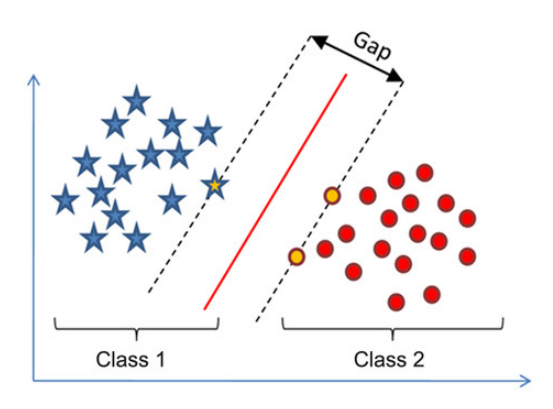
\includegraphics{esquema-basico-svm.PNG}
\caption{Figura 1: Ejemplo de 2 dimensiones para una máquina de soporte
vectorial, obsérvese que la recta roja es la que maximiza la distancia
entre los vectores de soporte (los puntos en amarillo)}
\end{figure}

Los universos a estudiar no se suelen presentar en casos idílicos de dos
dimensiones como en el ejemplo anterior, sino que un algoritmo SVM debe
tratar con:

\begin{itemize}
\tightlist
\item
  Más de dos variables predictoras
\item
  Curvas no lineales de separación
\item
  Casos donde los conjuntos de datos no pueden ser completamente
  separados
\item
  Clasificaciones en más de dos categorías
\end{itemize}

\begin{figure}[h]
\centering
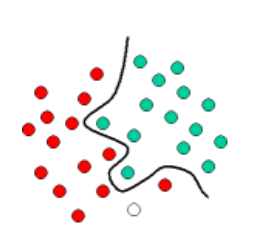
\includegraphics{no-separable-linealmente.PNG}
\caption{Figura 2: Espacio de 2 dimensiones en el que los patrones no
son separables linealmente}
\end{figure}

\subsection{Definición formal}\label{definiciuxf3n-formal}

\begin{quote}
Dado un conjunto de entrenamiento formado por pares de instancias y
etiquetas
\[(x_i,y_i),  i=1, . . . , l \text{ donde } x_i \in R^n, y \in \{1, −1\}^l\]
, las SVMs pueden entenderse como la solución al siguiente problema de
optimización:: \[
\begin{aligned}
\underset{w,b,\epsilon}{\operatorname{argmin}} & & \frac{1}{2}w^Tw + C
\sum_1^l{\epsilon_i} \\
\text{sujeto a} & & y_i(w^T \phi(x_i) + b) \ge 1- \epsilon_i \\
& & \epsilon_i \ge 0
\end{aligned}
\] Además, \[K(x_i, x_j ) ≡ \phi(x_i)^T \phi(x_j)\] es llamada la
función kernel.
\end{quote}

\emph{Figura 3. Definición formal de las SVMs según {[}4{]}}

Los vectores de entrenamiento \(x_i\) son asignados a un espacio de
mayor dimensiones (incluso infinitas) por la función \(\phi\). La
máquina de soporte vectorial encuentra el hiperplano con máximo margen
de separación en el espacio dimensional superior. C \textgreater{} 0 es
el parámetro de penalización del término de error.

\subsection{Funciones kernel}\label{funciones-kernel}

Cuando el espacio donde trabajamos no permite separar linealmente los
patrones de forma perfecta, como se puede observar en la figura 2, es
imposible trazar un hiperplano que separe perfectamente los patrones.

Por ello entran en juego las llamadas \textbf{funciones kernel},
funciones matemáticas que nos permiten proyectar los patrones en un
espacio de mayor dimensión que el original dónde estos si son
linealmente separables mediante un hiperplano (Figura 3).

\begin{figure}[h]
\centering
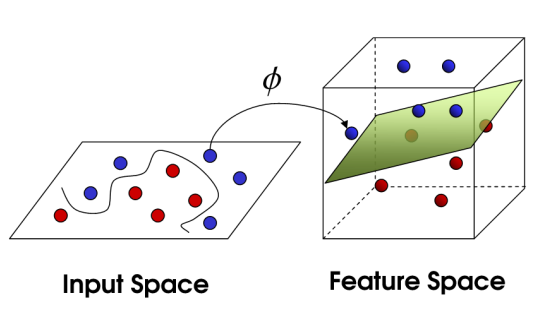
\includegraphics{ejemplo-kernel.PNG}
\caption{Figura 4: Kernel de 2 a 3 dimensiones dónde los patrones pueden
ser perfectamente separados mediante un hiperplano}
\end{figure}

De nuevo, y como en la gran mayoría de algoritmos de aprendizaje
máquina, \textbf{si elegimos un modelo (en este caso una función kernel)
que se ajuste demasiado bien a los patrones de entrenamiento}, el
clasificador perderá capacidad de generalización por lo que tendrá un
mal comportamiento ante nuevos patrones y se hablará de
\textbf{sobreentrenamiento}.

Las funciones kernel más comunmente utilizadas son:

\begin{itemize}
\tightlist
\item
  \textbf{lineales}:  
  $
  K(x_i,x_j) = x_i^{}T x_j 
  $
\item
  \textbf{polinómicas}:  
  $
  K(x_i,x_j) = (\gamma x_i^{}T x_j  +r)^{}d, \gamma \ge 0 $
\item
  \textbf{funciones de base radial (RBF)}:  
  $
  K(x_i,x_j) =
  exp(-\gamma \lvert x_i - x_j \lvert ^2), \gamma \ge 0
  $
\item
  \textbf{sigmoide}:  
  $
  K(x_i,x_j) = \tanh(\gamma x_i^T x_j +r)
  $
  
\end{itemize}

\subsection{Outliers}\label{outliers}

No siempre es posible encontrar una transformación de los datos que
permita separarlos linealmente {[}2{]} o incluso a veces, no es
conveniente.

En este caso nos encontramos con instancias en el conjunto de
entrenamiento que se situan en lugares del espacio muy separados o
aislados de la zona dónde se sitúan la mayoría de instancias de
entrenamiento con las que comparten la clase.

La presencia de ruido o de \textbf{outliers} pueden llegar tambien a
provocar soluciones sobreajustadas a los patrones de entrenamiento que
no generalizan bien. Para tratar con estas situaciones se crearon los
llamados \textbf{SVM de margen blando} cuya idea principal es introducir
una holgura al margen existente entre los vectores de soporte y el
hiperplano que permite que las restricciones no se cumplan de manera
estricta.

Se introduce por tanto en el proceso de entrenamiento una constante
\textbf{C} que controlará el tamaño de la holgura.

\textbf{El parámetro C le indica a la SVM, en el proceso de
entrenamiento, el grado de ejemplos mal clasificados permitido.}

Para valores grandes de C, la optimización elegirá un hiperplano de
margen más pequeño si ese hiperplano hace un mejor trabajo para
conseguir que todos los puntos de entrenamiento estén clasificados
correctamente. Es decir, se evitan en mayor medida ejemplos mal
clasificados aunque ello conduzca a hiperplanos de margen menor.

Por el contrario, un valor muy pequeño de C hará que el optimizador
busque un hiperplano de separación de mayor margen, incluso si ese
hiperplano clasifica erróneamente más puntos. Para valores muy pequeños
de C frecuentemente se obtienen ejemplos mal clasificados, incluso si
los datos de entrenamiento son linealmente separables. Sin embargo, el
sobreajuste del clasificador es menor y generalmente se obtienen
clasificadores que generalizan mejor.

\subsection{Preprocesado de datos}\label{preprocesado-de-datos}

Se suele realizar a dos niveles {[}4{]}:

\subsubsection{Atributos categóricos}\label{atributos-categuxf3ricos}

Las SVMs requieren que cada instancia de datos se represente como un
vector de números reales. Por lo tanto, si hay atributos categóricos,
primero tenemos que convertirlos en datos numéricos. Se recomienda
utilizar m números para representar un atributo con m categorías.
Solamente uno de los m números es uno, y los otros son cero. Por
ejemplo, una categoría de tres atributos como \{rojo, verde, azul\}
puede representarse como (0,0,1), (0,1,0) y (1,0,0).

La experiencia indica que si el número de valores en un atributo no es
demasiado grande, esta codificación puede ser más estable que usar un
solo número.

\subsubsection{Escalado}\label{escalado}

\textbf{Escalar los datos antes de aplicar las SVMs es muy importante.}
La mayoría de las consideraciones hechas para redes neuronales también
se aplican a las SVMs.

La principal ventaja de escalar es evitar que atributos cuyos valores se
mueven en rangos numéricos altos dominen a aquellos que se mueven en
rangos numéricos más pequeños. Otra ventaja es evitar dificultades
numéricas durante el cálculo, dado que los valores del kernel
normalmente dependen de los productos internos de vectores de
características, p.

Se recomienda un escalado lineal de cada atributo al rango {[}-1, +1{]}
o {[}0, 1{]}. Por supuesto, hay usar el mismo método para escalar el los
datos de entrenamiento y los de prueba.

\subsection{Selección del modelo}\label{selecciuxf3n-del-modelo}

Aunque sólo son cuatro las funciones kernel más comunes, se debe decidir
una para entrenar la SVM. Una vez elegido el núcleo, se ajustan los
parámetros de penalización C y los parámetros propios del kernel
elegido.

\textbf{Según {[}4{]}, en general, el núcleo RBF es una primera opción
razonable.}

Este kernel no correlaciona las muestras en un espacio dimensional
superior, a diferencia del núcleo lineal, con lo que se puede manejar el
caso cuando la relación entre las etiquetas y los atributos no es
lineal. Además, el núcleo lineal es un caso especial de RBF.

La segunda razón es el número de hiperparámetros que influyen en la
complejidad de la selección del modelo. El núcleo polinomial tiene más
hiperparametros que el núcleo RBF.

Por último, el núcleo RBF tiene menos dificultades numéricas ya que el
resultado de aplicar la función kernel es siempre menor que 1.

Hay algunas situaciones en las que el núcleo RBF no es adecuado. En
particular, cuando el número de características es muy grande, se puede
utilizar el núcleo lineal.

\subsection{Cross-validation}\label{cross-validation}

Aprender los parámetros de un modelo y probarlo en los mismos datos es
un error metodológico: un modelo que simplemente repitiera las etiquetas
de las muestras que acaba de ver tendría una puntuación perfecta pero no
podría predecir nada útil en otros datos no vistos. Esta situación se
conoce como \textbf{sobreajuste}. Para evitarlo, es una práctica común
cuando se realiza un experimento de aprendizaje (supervisado) mantener
una parte de los datos disponibles como un conjunto de pruebas.

Una solución a este problema es un procedimiento llamado
\textbf{validación cruzada} (CV para abreviar). Se guarda un conjunto de
prueba para la evaluación final, que no se utiliza en ningún caso en el
proceso de entrenamiento. En el enfoque básico, llamado \textbf{k-fold
CV}, el conjunto de entrenamiento se divide en k conjuntos más pequeños.
Se sigue el siguiente procedimiento para cada uno de los k ``bloques'',
en diversas iteraciones:

\begin{itemize}
\tightlist
\item
  El modelo es entrenado usando k-1 de los bloques
\item
  El modelo resultante se valida en el bloque restante no utilizado en
  esta iteración del entrenamiento
\item
  Este proceso se repite k veces (una para utilizando cada bloque como
  prueba)
\end{itemize}

Típicamente, la medida de rendimiento reportada por la validación
cruzada k-fold es el promedio de los valores calculados en las k
iteraciones. Este enfoque puede ser costoso desde el punto de vista
computacional, pero garantiza que los datos iniciales de prueba
realmente se utilizan sólo para las pruebas y que el entrenamiento puede
ser más productivo.

\section{Notas a la implementación}\label{notas-a-la-implementaciuxf3n}

En el enunciado de la práctica se hace mención explícita a WEKA y a
Torch.

Sin embargo, entiendo que el lenguaje o la herramienta con la que
resuelvan las prácticas es libre y las referencias a WEKA es simplemente
por tener una herramienta por defecto para quien no tenga otras
preferencias.

En este sentido, y espero no estar cometiendo un error, me tomo la
libertad de desarrollar esta práctica con python utilizando scikit-learn
como librería de machine-learning.

\section{Análisis del fichero s}\label{anuxe1lisis-del-fichero-s}

\subsection{Cargar los ficheros
s-train/test}\label{cargar-los-ficheros-s-traintest}

    \begingroup
\fontsize{8pt}{10pt}
\begin{mdframed}[hidealllines=true,backgroundcolor=blue!5]

\begin{Verbatim}[commandchars=\\\{\}]
\PY{k+kn}{from} \PY{n+nn}{scipy.io.arff} \PY{k+kn}{import} \PY{n}{loadarff}

\PY{n}{S\PYZus{}train}\PY{p}{,}\PY{n}{S\PYZus{}meta} \PY{o}{=} \PY{n}{loadarff}\PY{p}{(}\PY{l+s+s1}{\PYZsq{}}\PY{l+s+s1}{svm\PYZhy{}data/s\PYZhy{}train.arff}\PY{l+s+s1}{\PYZsq{}}\PY{p}{)}
\PY{n}{S\PYZus{}test}\PY{p}{,}\PY{n}{\PYZus{}}       \PY{o}{=} \PY{n}{loadarff}\PY{p}{(}\PY{l+s+s1}{\PYZsq{}}\PY{l+s+s1}{svm\PYZhy{}data/s\PYZhy{}test.arff}\PY{l+s+s1}{\PYZsq{}}\PY{p}{)} 
\end{Verbatim}

\end{mdframed}
\endgroup

    \subsection{Función de
normalización}\label{funciuxf3n-de-normalizaciuxf3n}

Tal como se ha indicado en la parte teórica de la práctica, es
fundamental normalizar los datos para obtener un correcto funcionamiento
de las SVM's, y por extensión de casi cualquier algoritmo de minería de
datos.

Aquí tenemos una función que nos hace todo el trabajo - \textbf{nótese
que normalizamos simultáneamente los datos de entrenamiento y de
prueba}. Sabemos que no aplicar el mismo tipo de normalización a los
datos con los que se prueba un modelo que a aquellos con los que se
entrena es tanto como probar el modelo con datos de otro dominio del que
estudia.

\hspace{0.5cm}
    \begingroup
\fontsize{8pt}{10pt}
\begin{mdframed}[hidealllines=true,backgroundcolor=blue!5]

\begin{Verbatim}[commandchars=\\\{\}]
\PY{k+kn}{from} \PY{n+nn}{sklearn.preprocessing} \PY{k+kn}{import} \PY{n}{normalize}

\PY{k}{def} \PY{n+nf}{normalize\PYZus{}data}\PY{p}{(}\PY{n}{train}\PY{p}{,} \PY{n}{test}\PY{p}{)}\PY{p}{:}
    \PY{l+s+sd}{\PYZdq{}\PYZdq{}\PYZdq{}Normaliza los datos de entrenamiento y prueba}
\PY{l+s+sd}{    y los devuelve como una tupla:}
\PY{l+s+sd}{    X\PYZus{}train,y\PYZus{}train,X\PYZus{}test,y\PYZus{}test}
\PY{l+s+sd}{    \PYZdq{}\PYZdq{}\PYZdq{}}
    \PY{n}{data} \PY{o}{=} \PY{n}{np}\PY{o}{.}\PY{n}{append}\PY{p}{(}\PY{n}{train}\PY{p}{,} \PY{n}{test}\PY{p}{)}
    \PY{n}{X} \PY{o}{=} \PY{n}{normalize}\PY{p}{(}\PY{p}{[}\PY{n+nb}{list}\PY{p}{(}\PY{n}{d}\PY{p}{)}\PY{p}{[}\PY{l+m+mi}{0}\PY{p}{:}\PY{o}{\PYZhy{}}\PY{l+m+mi}{1}\PY{p}{]} \PY{k}{for} \PY{n}{d} \PY{o+ow}{in} \PY{n}{data}\PY{p}{]}\PY{p}{,} \PY{n}{axis}\PY{o}{=}\PY{l+m+mi}{0}\PY{p}{)}
    \PY{n}{y} \PY{o}{=} \PY{p}{[}\PY{n+nb}{list}\PY{p}{(}\PY{n}{d}\PY{p}{)}\PY{p}{[}\PY{o}{\PYZhy{}}\PY{l+m+mi}{1}\PY{p}{]} \PY{k}{for} \PY{n}{d} \PY{o+ow}{in} \PY{n}{data}\PY{p}{]}
    \PY{n}{l} \PY{o}{=} \PY{n+nb}{len}\PY{p}{(}\PY{n}{train}\PY{p}{)}
    \PY{k}{return} \PY{n}{X}\PY{p}{[}\PY{p}{:}\PY{n}{l}\PY{p}{]}\PY{p}{,}\PY{n}{y}\PY{p}{[}\PY{p}{:}\PY{n}{l}\PY{p}{]}\PY{p}{,}\PY{n}{X}\PY{p}{[}\PY{n}{l}\PY{p}{:}\PY{p}{]}\PY{p}{,}\PY{n}{y}\PY{p}{[}\PY{n}{l}\PY{p}{:}\PY{p}{]} 
\end{Verbatim}

\end{mdframed}
\endgroup

    \subsection{Seleccionar las 3 clases más
frecuentes}\label{seleccionar-las-3-clases-muxe1s-frecuentes}

\hspace{0.5cm}
    \begingroup
\fontsize{8pt}{10pt}
\begin{mdframed}[hidealllines=true,backgroundcolor=blue!5]

\begin{Verbatim}[commandchars=\\\{\}]
\PY{k+kn}{import} \PY{n+nn}{numpy} \PY{k+kn}{as} \PY{n+nn}{np}


\PY{k}{def} \PY{n+nf}{top\PYZus{}three\PYZus{}categories}\PY{p}{(}\PY{n}{train}\PY{p}{,}\PY{n}{test}\PY{p}{)}\PY{p}{:}
    \PY{n}{classes} \PY{o}{=} \PY{n}{np}\PY{o}{.}\PY{n}{concatenate}\PY{p}{(}\PY{p}{(}\PY{n}{train}\PY{p}{[}\PY{l+s+s1}{\PYZsq{}}\PY{l+s+s1}{class}\PY{l+s+s1}{\PYZsq{}}\PY{p}{]}\PY{p}{,}\PY{n}{test}\PY{p}{[}\PY{l+s+s1}{\PYZsq{}}\PY{l+s+s1}{class}\PY{l+s+s1}{\PYZsq{}}\PY{p}{]}\PY{p}{)}\PY{p}{)}
    \PY{n}{class\PYZus{}counts} \PY{o}{=} \PY{n+nb}{dict}\PY{p}{(}\PY{n+nb}{zip}\PY{p}{(}\PY{o}{*}\PY{n}{np}\PY{o}{.}\PY{n}{unique}\PY{p}{(}\PY{n}{classes}\PY{p}{,}\PY{n}{return\PYZus{}counts}\PY{o}{=}\PY{n+nb+bp}{True}\PY{p}{)}\PY{p}{)}\PY{p}{)}
    \PY{n}{top\PYZus{}three} \PY{o}{=} \PY{n+nb}{sorted}\PY{p}{(}\PY{n}{class\PYZus{}counts}\PY{p}{,} \PY{n}{key}\PY{o}{=}\PY{n}{class\PYZus{}counts}\PY{o}{.}\PY{n}{get}\PY{p}{,} \PY{n}{reverse}\PY{o}{=}\PY{n+nb+bp}{True}\PY{p}{)}\PY{p}{[}\PY{l+m+mi}{0}\PY{p}{:}\PY{l+m+mi}{3}\PY{p}{]}
    \PY{k}{print} \PY{l+s+s1}{\PYZsq{}}\PY{l+s+s1}{Top 3 classes: }\PY{l+s+si}{\PYZpc{}s}\PY{l+s+s1}{\PYZsq{}} \PY{o}{\PYZpc{}} \PY{n}{top\PYZus{}three}
    \PY{k}{return} \PY{n}{train}\PY{p}{[}\PY{n}{np}\PY{o}{.}\PY{n}{in1d}\PY{p}{(}\PY{n}{train}\PY{p}{[}\PY{l+s+s1}{\PYZsq{}}\PY{l+s+s1}{class}\PY{l+s+s1}{\PYZsq{}}\PY{p}{]}\PY{p}{,} \PY{n}{top\PYZus{}three}\PY{p}{)}\PY{p}{]}\PY{p}{,}\PY{n}{test}\PY{p}{[}\PY{n}{np}\PY{o}{.}\PY{n}{in1d}\PY{p}{(}\PY{n}{test}\PY{p}{[}\PY{l+s+s1}{\PYZsq{}}\PY{l+s+s1}{class}\PY{l+s+s1}{\PYZsq{}}\PY{p}{]}\PY{p}{,} \PY{n}{top\PYZus{}three}\PY{p}{)}\PY{p}{]}

\PY{n}{S\PYZus{}top3\PYZus{}train}\PY{p}{,}\PY{n}{S\PYZus{}top3\PYZus{}test} \PY{o}{=} \PY{n}{top\PYZus{}three\PYZus{}categories}\PY{p}{(}\PY{n}{S\PYZus{}train}\PY{p}{,}\PY{n}{S\PYZus{}test}\PY{p}{)} 
\end{Verbatim}

\end{mdframed}
\endgroup

    \begin{Verbatim}[commandchars=\\\{\}]
Top 3 classes: ['46', '20', '110']

    \end{Verbatim}

    \subsection{Obtención de un clasificador MVS lineal en el espacio de
parámetros}\label{obtenciuxf3n-de-un-clasificador-mvs-lineal-en-el-espacio-de-paruxe1metros}

Vamos a realizar una búsqueda en el espacio de parámetros para
seleccionar el que produce mejores resultados evaluados mediante
validación cruzada.

Según las indicacione de la práctica, probaremos unos 20 valores de
\textbf{C entre 0.001 y 10}. Pero en lugar de utilizarlos equiespaciados
en escala lineal, creo que será más productivo (ofrecerá mejor ámbito
exploratorio) si los \textbf{equiespaciamos en escala logarítmica}.

\hspace{0.5cm}

    \begingroup
\fontsize{8pt}{10pt}
\begin{mdframed}[hidealllines=true,backgroundcolor=blue!5]

\begin{Verbatim}[commandchars=\\\{\}]
\PY{k+kn}{from} \PY{n+nn}{sklearn.model\PYZus{}selection} \PY{k+kn}{import} \PY{n}{GridSearchCV}
\PY{n}{np}\PY{o}{.}\PY{n}{set\PYZus{}printoptions}\PY{p}{(}\PY{n}{formatter}\PY{o}{=}\PY{p}{\PYZob{}}\PY{l+s+s1}{\PYZsq{}}\PY{l+s+s1}{float}\PY{l+s+s1}{\PYZsq{}}\PY{p}{:} \PY{k}{lambda} \PY{n}{x}\PY{p}{:} \PY{l+s+s2}{\PYZdq{}}\PY{l+s+s2}{\PYZob{}0:0.3f\PYZcb{}}\PY{l+s+s2}{\PYZdq{}}\PY{o}{.}\PY{n}{format}\PY{p}{(}\PY{n}{x}\PY{p}{)}\PY{p}{\PYZcb{}}\PY{p}{)}
    
\PY{n}{N} \PY{o}{=} \PY{l+m+mi}{20}
\PY{n}{Cs} \PY{o}{=} \PY{n}{np}\PY{o}{.}\PY{n}{logspace}\PY{p}{(}\PY{o}{\PYZhy{}}\PY{l+m+mi}{3}\PY{p}{,} \PY{l+m+mi}{1}\PY{p}{,} \PY{n}{N}\PY{p}{)}
\PY{k}{print} \PY{l+s+s1}{\PYZsq{}}\PY{l+s+s1}{Cs: }\PY{l+s+si}{\PYZpc{}s}\PY{l+s+s1}{\PYZsq{}} \PY{o}{\PYZpc{}} \PY{n}{Cs} 
\end{Verbatim}

\end{mdframed}
\endgroup

    \begin{Verbatim}[commandchars=\\\{\}]
Cs: [0.001 0.002 0.003 0.004 0.007 0.011 0.018 0.030 0.048 0.078 0.127 0.207
 0.336 0.546 0.886 1.438 2.336 3.793 6.158 10.000]

    \end{Verbatim}

    Vamos a utilizar además una búsqueda exhaustiva en el conjunto de Cs
anterior con la clase \textbf{GridSearchCV}.

\textbf{Esta función realiza automáticamente el entrenamiento con
cross-validation.} Por defecto utiliza 3 folds, y por defecto lo dejo,
ya que probando con otros no se obtienen resultados mucho mejores.

Después, obtendremos la información que necesitamos simplemente llamando
a los miembros:

\begin{itemize}
\tightlist
\item
  \textbf{best\_estimator\_} : el modelo que ofreció los mejores
  resultados de todos los probados
\item
  \textbf{best\_score\_} : la puntuación del mejor modelo indicado en el
  punto anterior
\end{itemize}
\hspace{0.5cm}
    \begingroup
\fontsize{8pt}{10pt}
\begin{mdframed}[hidealllines=true,backgroundcolor=blue!5]

\begin{Verbatim}[commandchars=\\\{\}]
\PY{k+kn}{from} \PY{n+nn}{sklearn} \PY{k+kn}{import} \PY{n}{svm}
\PY{k+kn}{from} \PY{n+nn}{sklearn.model\PYZus{}selection} \PY{k+kn}{import} \PY{n}{GridSearchCV}

\PY{n}{X\PYZus{}train}\PY{p}{,}\PY{n}{y\PYZus{}train}\PY{p}{,}\PY{n}{X\PYZus{}test}\PY{p}{,}\PY{n}{y\PYZus{}test} \PY{o}{=} \PY{n}{normalize\PYZus{}data}\PY{p}{(}\PY{n}{S\PYZus{}top3\PYZus{}train}\PY{p}{,}\PY{n}{S\PYZus{}top3\PYZus{}test}\PY{p}{)}
\PY{n}{gscv} \PY{o}{=} \PY{n}{GridSearchCV}\PY{p}{(}\PY{n}{estimator}\PY{o}{=}\PY{n}{svm}\PY{o}{.}\PY{n}{SVC}\PY{p}{(}\PY{n}{kernel}\PY{o}{=}\PY{l+s+s1}{\PYZsq{}}\PY{l+s+s1}{linear}\PY{l+s+s1}{\PYZsq{}}\PY{p}{)}\PY{p}{,} 
                    \PY{n}{param\PYZus{}grid}\PY{o}{=}\PY{n+nb}{dict}\PY{p}{(}\PY{n}{C}\PY{o}{=}\PY{n}{Cs}\PY{p}{)}\PY{p}{,} \PY{n}{n\PYZus{}jobs}\PY{o}{=}\PY{o}{\PYZhy{}}\PY{l+m+mi}{1}\PY{p}{)}
\PY{n}{gscv}\PY{o}{.}\PY{n}{fit}\PY{p}{(}\PY{n}{X\PYZus{}train}\PY{p}{,} \PY{n}{y\PYZus{}train}\PY{p}{)}

\PY{k}{print} \PY{l+s+s1}{\PYZsq{}}\PY{l+s+s1}{Mejor C: }\PY{l+s+si}{\PYZpc{}s}\PY{l+s+s1}{\PYZsq{}} \PY{o}{\PYZpc{}} \PY{n}{gscv}\PY{o}{.}\PY{n}{best\PYZus{}estimator\PYZus{}}\PY{o}{.}\PY{n}{C}
\PY{k}{print} \PY{l+s+s1}{\PYZsq{}}\PY{l+s+s1}{Puntuación del mejor modelo: }\PY{l+s+si}{\PYZpc{}s}\PY{l+s+s1}{\PYZsq{}} \PY{o}{\PYZpc{}} \PY{n}{gscv}\PY{o}{.}\PY{n}{best\PYZus{}score\PYZus{}} 
\end{Verbatim}

\end{mdframed}
\endgroup

    \begin{Verbatim}[commandchars=\\\{\}]
Mejor C: 10.0
Puntuación del mejor modelo: 0.835616438356

    \end{Verbatim}

    Como el mejor C enontrado se corresponde con el extremo derecho de los
probados en nuestro \textbf{grid}, vamos a aumentar el intervalo de
prueba por la derecha:

\hspace{0.5cm}

    \begingroup
\fontsize{8pt}{10pt}
\begin{mdframed}[hidealllines=true,backgroundcolor=blue!5]

\begin{Verbatim}[commandchars=\\\{\}]
\PY{n}{Cs} \PY{o}{=} \PY{n}{np}\PY{o}{.}\PY{n}{logspace}\PY{p}{(}\PY{l+m+mi}{1}\PY{p}{,} \PY{l+m+mi}{3}\PY{p}{,} \PY{n}{N}\PY{p}{)}
\PY{k}{print} \PY{l+s+s2}{\PYZdq{}}\PY{l+s+s2}{Cs: }\PY{l+s+si}{\PYZpc{}s}\PY{l+s+s2}{\PYZdq{}} \PY{o}{\PYZpc{}} \PY{n}{Cs}

\PY{n}{gscv} \PY{o}{=} \PY{n}{GridSearchCV}\PY{p}{(}\PY{n}{estimator}\PY{o}{=}\PY{n}{svm}\PY{o}{.}\PY{n}{SVC}\PY{p}{(}\PY{n}{kernel}\PY{o}{=}\PY{l+s+s1}{\PYZsq{}}\PY{l+s+s1}{linear}\PY{l+s+s1}{\PYZsq{}}\PY{p}{)}\PY{p}{,} 
                   \PY{n}{param\PYZus{}grid}\PY{o}{=}\PY{n+nb}{dict}\PY{p}{(}\PY{n}{C}\PY{o}{=}\PY{n}{Cs}\PY{p}{)}\PY{p}{,} \PY{n}{n\PYZus{}jobs}\PY{o}{=}\PY{o}{\PYZhy{}}\PY{l+m+mi}{1}\PY{p}{)}
\PY{n}{gscv}\PY{o}{.}\PY{n}{fit}\PY{p}{(}\PY{n}{X\PYZus{}train}\PY{p}{,} \PY{n}{y\PYZus{}train}\PY{p}{)}
\PY{k}{print} \PY{l+s+s1}{\PYZsq{}}\PY{l+s+s1}{Mejor C: }\PY{l+s+si}{\PYZpc{}s}\PY{l+s+s1}{\PYZsq{}} \PY{o}{\PYZpc{}} \PY{n}{gscv}\PY{o}{.}\PY{n}{best\PYZus{}estimator\PYZus{}}\PY{o}{.}\PY{n}{C}
\PY{k}{print} \PY{l+s+s1}{\PYZsq{}}\PY{l+s+s1}{Puntuación del mejor modelo: }\PY{l+s+si}{\PYZpc{}s}\PY{l+s+s1}{\PYZsq{}} \PY{o}{\PYZpc{}} \PY{n}{gscv}\PY{o}{.}\PY{n}{best\PYZus{}estimator\PYZus{}}\PY{o}{.}\PY{n}{score}\PY{p}{(}\PY{n}{X\PYZus{}test}\PY{p}{,} \PY{n}{y\PYZus{}test}\PY{p}{)} 
\end{Verbatim}

\end{mdframed}
\endgroup

    \begin{Verbatim}[commandchars=\\\{\}]
Cs: [10.000 12.743 16.238 20.691 26.367 33.598 42.813 54.556 69.519 88.587
 112.884 143.845 183.298 233.572 297.635 379.269 483.293 615.848 784.760
 1000.000]
Mejor C: 183.298071083
Puntuación del mejor modelo: 0.90756302521

    \end{Verbatim}

    Aunque el rendimiento de esta SVM es bastante bueno (90\%), resulta
bastante incómodo que el valor C sea tan grande. Es decir, el mejor
modelo encontrado \textbf{es de margen muy rígido}, lo que puede sugerir
que el modelo está sobreajustado.

Para disipar esta duda, podemos hacer el mismo experimento pero probando
con un valor más blando y ver si se obtienen resultados parecidos.

\hspace{0.5cm}

    \begingroup
\fontsize{8pt}{10pt}
\begin{mdframed}[hidealllines=true,backgroundcolor=blue!5]

\begin{Verbatim}[commandchars=\\\{\}]
\PY{n}{gscv} \PY{o}{=} \PY{n}{GridSearchCV}\PY{p}{(}\PY{n}{estimator}\PY{o}{=}\PY{n}{svm}\PY{o}{.}\PY{n}{SVC}\PY{p}{(}\PY{n}{kernel}\PY{o}{=}\PY{l+s+s1}{\PYZsq{}}\PY{l+s+s1}{linear}\PY{l+s+s1}{\PYZsq{}}\PY{p}{)}\PY{p}{,} 
                   \PY{n}{param\PYZus{}grid}\PY{o}{=}\PY{n+nb}{dict}\PY{p}{(}\PY{n}{C}\PY{o}{=}\PY{p}{[}\PY{l+m+mf}{0.1}\PY{p}{]}\PY{p}{)}\PY{p}{,} \PY{n}{n\PYZus{}jobs}\PY{o}{=}\PY{o}{\PYZhy{}}\PY{l+m+mi}{1}\PY{p}{)}
\PY{n}{gscv}\PY{o}{.}\PY{n}{fit}\PY{p}{(}\PY{n}{X\PYZus{}train}\PY{p}{,} \PY{n}{y\PYZus{}train}\PY{p}{)}
\PY{k}{print} \PY{l+s+s1}{\PYZsq{}}\PY{l+s+s1}{Puntuación del modelo con C=0.1: }\PY{l+s+si}{\PYZpc{}s}\PY{l+s+s1}{\PYZsq{}} \PY{o}{\PYZpc{}} \PY{n}{gscv}\PY{o}{.}\PY{n}{best\PYZus{}estimator\PYZus{}}\PY{o}{.}\PY{n}{score}\PY{p}{(}\PY{n}{X\PYZus{}test}\PY{p}{,} \PY{n}{y\PYZus{}test}\PY{p}{)} 
\end{Verbatim}

\end{mdframed}
\endgroup

    \begin{Verbatim}[commandchars=\\\{\}]
Puntuación del modelo con C=0.1: 0.36974789916

    \end{Verbatim}

    \textbf{Aunque hemos encontrado una máquina que ofrece unos resultados
de clasificación en torno al 0.90\%, el parámetro de penalización de los
errores de clasificación de la misma es altísimo, C=183. Sin embargo,
probando coma un valor C=0.1 más pequeño, vemos que el rendimiento de la
máquina obtenida es muy pequeño. Por lo tanto, entiendo que esto nos
invita a pensar que el problema NO es linealmente separable.} Sería
linealmente separable si obtuviéramos buenos resultados de clasificación
con una máquina de margen blando (C próximo a 0).

    \subsection{Realizar una búsqueda similar para núcleos polinómicos de
grado
2}\label{realizar-una-buxfasqueda-similar-para-nuxfacleos-polinuxf3micos-de-grado-2}

Procedemos de forma similar al punto anterior, pero en este caso
utilizando una función kernel de tipo polinómica.

\hspace{0.5cm}

    \begingroup
\fontsize{8pt}{10pt}
\begin{mdframed}[hidealllines=true,backgroundcolor=blue!5]

\begin{Verbatim}[commandchars=\\\{\}]
\PY{n}{N} \PY{o}{=} \PY{l+m+mi}{20}
\PY{n}{Cs} \PY{o}{=} \PY{n}{np}\PY{o}{.}\PY{n}{logspace}\PY{p}{(}\PY{o}{\PYZhy{}}\PY{l+m+mi}{3}\PY{p}{,} \PY{l+m+mi}{1}\PY{p}{,} \PY{n}{N}\PY{p}{)}
\PY{n}{Gs} \PY{o}{=} \PY{n}{np}\PY{o}{.}\PY{n}{logspace}\PY{p}{(}\PY{o}{\PYZhy{}}\PY{l+m+mi}{3}\PY{p}{,} \PY{l+m+mi}{1}\PY{p}{,} \PY{n}{N}\PY{p}{)}

\PY{k}{for} \PY{n}{n} \PY{o+ow}{in} \PY{n+nb}{range}\PY{p}{(}\PY{l+m+mi}{1}\PY{p}{,}\PY{l+m+mi}{5}\PY{p}{)}\PY{p}{:}  \PY{c+c1}{\PYZsh{} Probamos hasta grado 5}
    \PY{n}{gscv} \PY{o}{=} \PY{n}{GridSearchCV}\PY{p}{(}\PY{n}{estimator}\PY{o}{=}\PY{n}{svm}\PY{o}{.}\PY{n}{SVC}\PY{p}{(}\PY{n}{kernel}\PY{o}{=}\PY{l+s+s1}{\PYZsq{}}\PY{l+s+s1}{poly}\PY{l+s+s1}{\PYZsq{}}\PY{p}{,} \PY{n}{degree}\PY{o}{=}\PY{n}{n}\PY{p}{)}\PY{p}{,} 
                        \PY{n}{param\PYZus{}grid}\PY{o}{=}\PY{n+nb}{dict}\PY{p}{(}\PY{n}{C}\PY{o}{=}\PY{n}{Cs}\PY{p}{,}\PY{n}{gamma}\PY{o}{=}\PY{n}{Gs}\PY{p}{)}\PY{p}{,} \PY{n}{n\PYZus{}jobs}\PY{o}{=}\PY{o}{\PYZhy{}}\PY{l+m+mi}{1}\PY{p}{)}
    \PY{n}{gscv}\PY{o}{.}\PY{n}{fit}\PY{p}{(}\PY{n}{X\PYZus{}train}\PY{p}{,} \PY{n}{y\PYZus{}train}\PY{p}{)}
    \PY{k}{print} \PY{l+s+s1}{\PYZsq{}}\PY{l+s+s1}{Con grado }\PY{l+s+si}{\PYZpc{}s}\PY{l+s+s1}{\PYZsq{}} \PY{o}{\PYZpc{}} \PY{n}{n}
    \PY{k}{print} \PY{l+s+s1}{\PYZsq{}}\PY{l+s+s1}{Mejor C: }\PY{l+s+si}{\PYZpc{}s}\PY{l+s+s1}{\PYZsq{}} \PY{o}{\PYZpc{}} \PY{n}{gscv}\PY{o}{.}\PY{n}{best\PYZus{}estimator\PYZus{}}\PY{o}{.}\PY{n}{C}
    \PY{k}{print} \PY{l+s+s1}{\PYZsq{}}\PY{l+s+s1}{Mejor gamma: }\PY{l+s+si}{\PYZpc{}s}\PY{l+s+s1}{\PYZsq{}} \PY{o}{\PYZpc{}} \PY{n}{gscv}\PY{o}{.}\PY{n}{best\PYZus{}estimator\PYZus{}}\PY{o}{.}\PY{n}{gamma}
    \PY{k}{print} \PY{l+s+s1}{\PYZsq{}}\PY{l+s+s1}{Puntuación del mejor modelo: }\PY{l+s+si}{\PYZpc{}s}\PY{l+s+s1}{\PYZsq{}} \PY{o}{\PYZpc{}} \PY{n}{gscv}\PY{o}{.}\PY{n}{best\PYZus{}estimator\PYZus{}}\PY{o}{.}\PY{n}{score}\PY{p}{(}\PY{n}{X\PYZus{}test}\PY{p}{,} \PY{n}{y\PYZus{}test}\PY{p}{)} 
\end{Verbatim}

\end{mdframed}
\endgroup

    \begin{Verbatim}[commandchars=\\\{\}]
Con grado 1
Mejor C: 10.0
Mejor gamma: 10.0
Puntuación del mejor modelo: 0.890756302521
Con grado 2
Mejor C: 10.0
Mejor gamma: 10.0
Puntuación del mejor modelo: 0.90756302521
Con grado 3
Mejor C: 3.79269019073
Mejor gamma: 10.0
Puntuación del mejor modelo: 0.915966386555
Con grado 4
Mejor C: 3.79269019073
Mejor gamma: 10.0
Puntuación del mejor modelo: 0.90756302521

    \end{Verbatim}

    Vemos que obtenemos una máquina capaz de clasificar el 91\% de las
instancias con un C=3.79, es decir, de margen blando.

\subsection{Obtención de un clasificador MVS lineal en el espacio
proyectado mediante un núcleo
gaussiano}\label{obtenciuxf3n-de-un-clasificador-mvs-lineal-en-el-espacio-proyectado-mediante-un-nuxfacleo-gaussiano}

Repetimos los pasos del apartado anterior incluyendo en la ventana de
parámetros explorados dos entradas, una para el parámetro C y otra para
G (gamma) del núcleo gaussiano o de base radial.

\hspace{0.5cm}

    \begingroup
\fontsize{8pt}{10pt}
\begin{mdframed}[hidealllines=true,backgroundcolor=blue!5]

\begin{Verbatim}[commandchars=\\\{\}]
\PY{n}{N} \PY{o}{=} \PY{l+m+mi}{20}
\PY{n}{Cs} \PY{o}{=} \PY{n}{np}\PY{o}{.}\PY{n}{logspace}\PY{p}{(}\PY{o}{\PYZhy{}}\PY{l+m+mi}{3}\PY{p}{,} \PY{l+m+mi}{1}\PY{p}{,} \PY{n}{N}\PY{p}{)}
\PY{n}{Gs} \PY{o}{=} \PY{n}{np}\PY{o}{.}\PY{n}{logspace}\PY{p}{(}\PY{o}{\PYZhy{}}\PY{l+m+mi}{3}\PY{p}{,} \PY{l+m+mi}{1}\PY{p}{,} \PY{n}{N}\PY{p}{)}
\PY{n}{gscv} \PY{o}{=} \PY{n}{GridSearchCV}\PY{p}{(}\PY{n}{estimator}\PY{o}{=}\PY{n}{svm}\PY{o}{.}\PY{n}{SVC}\PY{p}{(}\PY{n}{kernel}\PY{o}{=}\PY{l+s+s1}{\PYZsq{}}\PY{l+s+s1}{rbf}\PY{l+s+s1}{\PYZsq{}}\PY{p}{)}\PY{p}{,} 
                    \PY{n}{param\PYZus{}grid}\PY{o}{=}\PY{n+nb}{dict}\PY{p}{(}\PY{n}{C}\PY{o}{=}\PY{n}{Cs}\PY{p}{,} \PY{n}{gamma}\PY{o}{=}\PY{n}{Gs}\PY{p}{)}\PY{p}{,} \PY{n}{n\PYZus{}jobs}\PY{o}{=}\PY{o}{\PYZhy{}}\PY{l+m+mi}{1}\PY{p}{)}
\PY{n}{gscv}\PY{o}{.}\PY{n}{fit}\PY{p}{(}\PY{n}{X\PYZus{}train}\PY{p}{,} \PY{n}{y\PYZus{}train}\PY{p}{)}
\PY{k}{print} \PY{l+s+s1}{\PYZsq{}}\PY{l+s+s1}{Mejor C: }\PY{l+s+si}{\PYZpc{}s}\PY{l+s+s1}{\PYZsq{}} \PY{o}{\PYZpc{}} \PY{n}{gscv}\PY{o}{.}\PY{n}{best\PYZus{}estimator\PYZus{}}\PY{o}{.}\PY{n}{C}
\PY{k}{print} \PY{l+s+s1}{\PYZsq{}}\PY{l+s+s1}{Mejor gamma: }\PY{l+s+si}{\PYZpc{}s}\PY{l+s+s1}{\PYZsq{}} \PY{o}{\PYZpc{}} \PY{n}{gscv}\PY{o}{.}\PY{n}{best\PYZus{}estimator\PYZus{}}\PY{o}{.}\PY{n}{gamma}
\PY{k}{print} \PY{l+s+s1}{\PYZsq{}}\PY{l+s+s1}{Puntuación del mejor modelo: }\PY{l+s+si}{\PYZpc{}s}\PY{l+s+s1}{\PYZsq{}} \PY{o}{\PYZpc{}} \PY{n}{gscv}\PY{o}{.}\PY{n}{best\PYZus{}estimator\PYZus{}}\PY{o}{.}\PY{n}{score}\PY{p}{(}\PY{n}{X\PYZus{}test}\PY{p}{,} \PY{n}{y\PYZus{}test}\PY{p}{)} 
\end{Verbatim}

\end{mdframed}
\endgroup

    \begin{Verbatim}[commandchars=\\\{\}]
Mejor C: 3.79269019073
Mejor gamma: 3.79269019073
Puntuación del mejor modelo: 0.873949579832

    \end{Verbatim}

    En este caso observamos que aunque el scoring obtenido por el mejor
modelo encontrado es similar al mejor encontrado en el caso anterior, el
parámetro gamma es inferior. Entiendo que podemos pensar que para este
conjunto de datos, SVMs basadas en núcleos gausianos son más apropiadas.

    \section{Probar distintos tipos de nucleos con un problema no separable
linealmente}\label{probar-distintos-tipos-de-nucleos-con-un-problema-no-separable-linealmente}

Definimos unas funciones que nos permita dibujar los datos y las curvas
de decisión de los clasificadores obtenidos en cada experimento.

\hspace{0.5cm}

    \begingroup
\fontsize{8pt}{10pt}
\begin{mdframed}[hidealllines=true,backgroundcolor=blue!5]

\begin{Verbatim}[commandchars=\\\{\}]
\PY{o}{\PYZpc{}}\PY{k}{matplotlib} inline 
\PY{k+kn}{from} \PY{n+nn}{matplotlib} \PY{k+kn}{import} \PY{n}{pyplot} \PY{k}{as} \PY{n}{plt}

\PY{k}{def} \PY{n+nf}{plot\PYZus{}data}\PY{p}{(}\PY{n}{data}\PY{p}{)}\PY{p}{:}
    \PY{n}{plt}\PY{o}{.}\PY{n}{figure}\PY{p}{(}\PY{n}{figsize}\PY{o}{=}\PY{p}{(}\PY{l+m+mi}{6}\PY{p}{,} \PY{l+m+mi}{4}\PY{p}{)}\PY{p}{)}
    \PY{n}{trues} \PY{o}{=} \PY{n}{data}\PY{p}{[}\PY{n}{data}\PY{p}{[}\PY{p}{:}\PY{p}{,}\PY{l+m+mi}{2}\PY{p}{]} \PY{o}{==} \PY{n+nb+bp}{True}\PY{p}{]}
    \PY{n}{plt}\PY{o}{.}\PY{n}{plot}\PY{p}{(}\PY{n}{trues}\PY{p}{[}\PY{p}{:}\PY{p}{,}\PY{l+m+mi}{0}\PY{p}{]}\PY{p}{,} \PY{n}{trues}\PY{p}{[}\PY{p}{:}\PY{p}{,}\PY{l+m+mi}{1}\PY{p}{]}\PY{p}{,} \PY{l+s+s1}{\PYZsq{}}\PY{l+s+s1}{bo}\PY{l+s+s1}{\PYZsq{}}\PY{p}{,} \PY{n}{markersize}\PY{o}{=}\PY{l+m+mi}{2}\PY{p}{)}
    \PY{n}{falses} \PY{o}{=} \PY{n}{data}\PY{p}{[}\PY{n}{data}\PY{p}{[}\PY{p}{:}\PY{p}{,}\PY{l+m+mi}{2}\PY{p}{]} \PY{o}{==} \PY{n+nb+bp}{False}\PY{p}{]}
    \PY{n}{plt}\PY{o}{.}\PY{n}{plot}\PY{p}{(}\PY{n}{falses}\PY{p}{[}\PY{p}{:}\PY{p}{,}\PY{l+m+mi}{0}\PY{p}{]}\PY{p}{,} \PY{n}{falses}\PY{p}{[}\PY{p}{:}\PY{p}{,}\PY{l+m+mi}{1}\PY{p}{]}\PY{p}{,} \PY{l+s+s1}{\PYZsq{}}\PY{l+s+s1}{ro}\PY{l+s+s1}{\PYZsq{}}\PY{p}{,} \PY{n}{markersize}\PY{o}{=}\PY{l+m+mi}{2}\PY{p}{)}
    \PY{n}{plt}\PY{o}{.}\PY{n}{show}\PY{p}{(}\PY{p}{)}
    
\PY{k}{def} \PY{n+nf}{plot\PYZus{}decision\PYZus{}function}\PY{p}{(}\PY{n}{clf}\PY{p}{,} \PY{n}{X}\PY{p}{,} \PY{n}{y}\PY{p}{)}\PY{p}{:}
    \PY{n}{h} \PY{o}{=} \PY{o}{.}\PY{l+m+mi}{1}  \PY{c+c1}{\PYZsh{} step size in the mesh}
    \PY{n}{x\PYZus{}min}\PY{p}{,} \PY{n}{x\PYZus{}max} \PY{o}{=} \PY{n}{X}\PY{p}{[}\PY{p}{:}\PY{p}{,} \PY{l+m+mi}{0}\PY{p}{]}\PY{o}{.}\PY{n}{min}\PY{p}{(}\PY{p}{)} \PY{o}{\PYZhy{}} \PY{l+m+mi}{1}\PY{p}{,} \PY{n}{X}\PY{p}{[}\PY{p}{:}\PY{p}{,} \PY{l+m+mi}{0}\PY{p}{]}\PY{o}{.}\PY{n}{max}\PY{p}{(}\PY{p}{)} \PY{o}{+} \PY{l+m+mi}{1}
    \PY{n}{y\PYZus{}min}\PY{p}{,} \PY{n}{y\PYZus{}max} \PY{o}{=} \PY{n}{X}\PY{p}{[}\PY{p}{:}\PY{p}{,} \PY{l+m+mi}{1}\PY{p}{]}\PY{o}{.}\PY{n}{min}\PY{p}{(}\PY{p}{)} \PY{o}{\PYZhy{}} \PY{l+m+mi}{1}\PY{p}{,} \PY{n}{X}\PY{p}{[}\PY{p}{:}\PY{p}{,} \PY{l+m+mi}{1}\PY{p}{]}\PY{o}{.}\PY{n}{max}\PY{p}{(}\PY{p}{)} \PY{o}{+} \PY{l+m+mi}{1}
    \PY{n}{xx}\PY{p}{,} \PY{n}{yy} \PY{o}{=} \PY{n}{np}\PY{o}{.}\PY{n}{meshgrid}\PY{p}{(}\PY{n}{np}\PY{o}{.}\PY{n}{arange}\PY{p}{(}\PY{n}{x\PYZus{}min}\PY{p}{,} \PY{n}{x\PYZus{}max}\PY{p}{,} \PY{n}{h}\PY{p}{)}\PY{p}{,} 
                         \PY{n}{np}\PY{o}{.}\PY{n}{arange}\PY{p}{(}\PY{n}{y\PYZus{}min}\PY{p}{,} \PY{n}{y\PYZus{}max}\PY{p}{,} \PY{n}{h}\PY{p}{)}\PY{p}{)}
    \PY{n}{Z} \PY{o}{=} \PY{n}{clf}\PY{o}{.}\PY{n}{predict}\PY{p}{(}\PY{n}{np}\PY{o}{.}\PY{n}{c\PYZus{}}\PY{p}{[}\PY{n}{xx}\PY{o}{.}\PY{n}{ravel}\PY{p}{(}\PY{p}{)}\PY{p}{,} \PY{n}{yy}\PY{o}{.}\PY{n}{ravel}\PY{p}{(}\PY{p}{)}\PY{p}{]}\PY{p}{)}
    \PY{n}{Z} \PY{o}{=} \PY{n}{Z}\PY{o}{.}\PY{n}{reshape}\PY{p}{(}\PY{n}{xx}\PY{o}{.}\PY{n}{shape}\PY{p}{)}
    
    \PY{n}{plt}\PY{o}{.}\PY{n}{figure}\PY{p}{(}\PY{n}{figsize}\PY{o}{=}\PY{p}{(}\PY{l+m+mi}{6}\PY{p}{,} \PY{l+m+mi}{4}\PY{p}{)}\PY{p}{)}
    \PY{n}{plt}\PY{o}{.}\PY{n}{pcolormesh}\PY{p}{(}\PY{n}{xx}\PY{p}{,} \PY{n}{yy}\PY{p}{,} \PY{n}{Z}\PY{p}{,} \PY{n}{cmap}\PY{o}{=}\PY{n}{plt}\PY{o}{.}\PY{n}{cm}\PY{o}{.}\PY{n}{Paired}\PY{p}{)}
    \PY{n}{plt}\PY{o}{.}\PY{n}{title}\PY{p}{(}\PY{l+s+s1}{\PYZsq{}}\PY{l+s+s1}{Funcion de decision del modelo}\PY{l+s+s1}{\PYZsq{}}\PY{p}{)}
    \PY{n}{plt}\PY{o}{.}\PY{n}{axis}\PY{p}{(}\PY{l+s+s1}{\PYZsq{}}\PY{l+s+s1}{tight}\PY{l+s+s1}{\PYZsq{}}\PY{p}{)}
    \PY{n}{plt}\PY{o}{.}\PY{n}{show}\PY{p}{(}\PY{p}{)} 
\end{Verbatim}

\end{mdframed}
\endgroup

    \subsection{Gausianas con escaso solape - separables
linealmente}\label{gausianas-con-escaso-solape---separables-linealmente}

Utilizo dos distribuciones gausianas de 2 dimensione con medias bien
distintas.

\hspace{0.5cm}

    \begingroup
\fontsize{8pt}{10pt}
\begin{mdframed}[hidealllines=true,backgroundcolor=blue!5]

\begin{Verbatim}[commandchars=\\\{\}]
\PY{n}{x} \PY{o}{=} \PY{p}{[}\PY{p}{[}\PY{n}{a}\PY{p}{,}\PY{n}{b}\PY{p}{,}\PY{l+m+mi}{0}\PY{p}{]} \PY{k}{for} \PY{n}{a}\PY{p}{,}\PY{n}{b} \PY{o+ow}{in} \PY{n}{np}\PY{o}{.}\PY{n}{random}\PY{o}{.}\PY{n}{normal}\PY{p}{(}\PY{n}{loc}\PY{o}{=}\PY{o}{\PYZhy{}}\PY{l+m+mi}{2}\PY{p}{,} \PY{n}{size}\PY{o}{=}\PY{p}{(}\PY{l+m+mi}{1000}\PY{p}{,}\PY{l+m+mi}{2}\PY{p}{)}\PY{p}{)}\PY{p}{]}
\PY{n}{y} \PY{o}{=} \PY{p}{[}\PY{p}{[}\PY{n}{a}\PY{p}{,}\PY{n}{b}\PY{p}{,}\PY{l+m+mi}{1}\PY{p}{]} \PY{k}{for} \PY{n}{a}\PY{p}{,}\PY{n}{b} \PY{o+ow}{in} \PY{n}{np}\PY{o}{.}\PY{n}{random}\PY{o}{.}\PY{n}{normal}\PY{p}{(}\PY{n}{loc}\PY{o}{=}\PY{l+m+mi}{2}\PY{p}{,} \PY{n}{size}\PY{o}{=}\PY{p}{(}\PY{l+m+mi}{1000}\PY{p}{,}\PY{l+m+mi}{2}\PY{p}{)}\PY{p}{)}\PY{p}{]}
\PY{n}{data} \PY{o}{=} \PY{n}{np}\PY{o}{.}\PY{n}{concatenate}\PY{p}{(}\PY{p}{[}\PY{n}{x}\PY{p}{,}\PY{n}{y}\PY{p}{]}\PY{p}{)}
\PY{n}{np}\PY{o}{.}\PY{n}{random}\PY{o}{.}\PY{n}{shuffle}\PY{p}{(}\PY{n}{data}\PY{p}{)}
\PY{n}{X\PYZus{}train}\PY{p}{,} \PY{n}{y\PYZus{}train} \PY{o}{=} \PY{n}{data}\PY{p}{[}\PY{p}{:}\PY{l+m+mi}{1500}\PY{p}{,}\PY{p}{:}\PY{o}{\PYZhy{}}\PY{l+m+mi}{1}\PY{p}{]}\PY{p}{,} \PY{n}{data}\PY{p}{[}\PY{p}{:}\PY{l+m+mi}{1500}\PY{p}{,}\PY{o}{\PYZhy{}}\PY{l+m+mi}{1}\PY{p}{]} 
\PY{n}{X\PYZus{}test}\PY{p}{,} \PY{n}{y\PYZus{}test} \PY{o}{=} \PY{n}{data}\PY{p}{[}\PY{l+m+mi}{1500}\PY{p}{:}\PY{p}{,}\PY{p}{:}\PY{o}{\PYZhy{}}\PY{l+m+mi}{1}\PY{p}{]}\PY{p}{,} \PY{n}{data}\PY{p}{[}\PY{l+m+mi}{1500}\PY{p}{:}\PY{p}{,}\PY{o}{\PYZhy{}}\PY{l+m+mi}{1}\PY{p}{]}
\PY{n}{plot\PYZus{}data}\PY{p}{(}\PY{n}{data}\PY{p}{)} 
\end{Verbatim}

\end{mdframed}
\endgroup

    \begin{center}
    \adjustimage{max size={0.9\linewidth}{0.9\paperheight}}{p_24_0.png}
    \end{center}
    { \hspace*{\fill} \\}
    
    Gráficamente sé ve que este ejemplo sí es linealmente separable. Vamos a
confirmarlo encontrando una SVM con un buen rendimiento:

\hspace{0.5cm}

    \begingroup
\fontsize{8pt}{10pt}
\begin{mdframed}[hidealllines=true,backgroundcolor=blue!5]

\begin{Verbatim}[commandchars=\\\{\}]
\PY{n}{model} \PY{o}{=} \PY{n}{svm}\PY{o}{.}\PY{n}{SVC}\PY{p}{(}\PY{n}{kernel}\PY{o}{=}\PY{l+s+s1}{\PYZsq{}}\PY{l+s+s1}{linear}\PY{l+s+s1}{\PYZsq{}}\PY{p}{)}\PY{o}{.}\PY{n}{fit}\PY{p}{(}\PY{n}{X\PYZus{}train}\PY{p}{,}\PY{n}{y\PYZus{}train}\PY{p}{)}
\PY{k}{print} \PY{l+s+s1}{\PYZsq{}}\PY{l+s+s1}{Model C: }\PY{l+s+si}{\PYZpc{}s}\PY{l+s+s1}{\PYZsq{}} \PY{o}{\PYZpc{}} \PY{n}{model}\PY{o}{.}\PY{n}{C}
\PY{k}{print} \PY{l+s+s1}{\PYZsq{}}\PY{l+s+s1}{Model score: }\PY{l+s+si}{\PYZpc{}s}\PY{l+s+s1}{\PYZsq{}} \PY{o}{\PYZpc{}} \PY{n}{model}\PY{o}{.}\PY{n}{score}\PY{p}{(}\PY{n}{X\PYZus{}test}\PY{p}{,}\PY{n}{y\PYZus{}test}\PY{p}{)}
\PY{n}{plot\PYZus{}decision\PYZus{}function}\PY{p}{(}\PY{n}{model}\PY{p}{,} \PY{n}{X\PYZus{}train}\PY{p}{,} \PY{n}{y\PYZus{}train}\PY{p}{)} 
\end{Verbatim}

\end{mdframed}
\endgroup

    \begin{Verbatim}[commandchars=\\\{\}]
Model C: 1.0
Model score: 1.0

    \end{Verbatim}

    \begin{center}
    \adjustimage{max size={0.9\linewidth}{0.9\paperheight}}{p_26_1.png}
    \end{center}
    { \hspace*{\fill} \\}
    
    \subsection{Gausianas fuertemente solapadas - no
separables}\label{gausianas-fuertemente-solapadas---no-separables}

Utilizo dos distribuciones gausianas de 2 dimensione con medias no muy
distintas.

\hspace{0.5cm}

    \begingroup
\fontsize{8pt}{10pt}
\begin{mdframed}[hidealllines=true,backgroundcolor=blue!5]

\begin{Verbatim}[commandchars=\\\{\}]
\PY{n}{x} \PY{o}{=} \PY{p}{[}\PY{p}{[}\PY{n}{a}\PY{p}{,}\PY{n}{b}\PY{p}{,}\PY{l+m+mi}{0}\PY{p}{]} \PY{k}{for} \PY{n}{a}\PY{p}{,}\PY{n}{b} \PY{o+ow}{in} \PY{n}{np}\PY{o}{.}\PY{n}{random}\PY{o}{.}\PY{n}{normal}\PY{p}{(}\PY{n}{loc}\PY{o}{=}\PY{o}{\PYZhy{}}\PY{l+m+mf}{0.2}\PY{p}{,} \PY{n}{size}\PY{o}{=}\PY{p}{(}\PY{l+m+mi}{1000}\PY{p}{,}\PY{l+m+mi}{2}\PY{p}{)}\PY{p}{)}\PY{p}{]}
\PY{n}{y} \PY{o}{=} \PY{p}{[}\PY{p}{[}\PY{n}{a}\PY{p}{,}\PY{n}{b}\PY{p}{,}\PY{l+m+mi}{1}\PY{p}{]} \PY{k}{for} \PY{n}{a}\PY{p}{,}\PY{n}{b} \PY{o+ow}{in} \PY{n}{np}\PY{o}{.}\PY{n}{random}\PY{o}{.}\PY{n}{normal}\PY{p}{(}\PY{n}{loc}\PY{o}{=}\PY{l+m+mf}{0.2}\PY{p}{,} \PY{n}{size}\PY{o}{=}\PY{p}{(}\PY{l+m+mi}{1000}\PY{p}{,}\PY{l+m+mi}{2}\PY{p}{)}\PY{p}{)}\PY{p}{]}
\PY{n}{data} \PY{o}{=} \PY{n}{np}\PY{o}{.}\PY{n}{concatenate}\PY{p}{(}\PY{p}{[}\PY{n}{x}\PY{p}{,}\PY{n}{y}\PY{p}{]}\PY{p}{)}
\PY{n}{np}\PY{o}{.}\PY{n}{random}\PY{o}{.}\PY{n}{shuffle}\PY{p}{(}\PY{n}{data}\PY{p}{)}
\PY{n}{X\PYZus{}train}\PY{p}{,} \PY{n}{y\PYZus{}train} \PY{o}{=} \PY{n}{data}\PY{p}{[}\PY{p}{:}\PY{l+m+mi}{1500}\PY{p}{,}\PY{p}{:}\PY{o}{\PYZhy{}}\PY{l+m+mi}{1}\PY{p}{]}\PY{p}{,} \PY{n}{data}\PY{p}{[}\PY{p}{:}\PY{l+m+mi}{1500}\PY{p}{,}\PY{o}{\PYZhy{}}\PY{l+m+mi}{1}\PY{p}{]} 
\PY{n}{X\PYZus{}test}\PY{p}{,} \PY{n}{y\PYZus{}test} \PY{o}{=} \PY{n}{data}\PY{p}{[}\PY{l+m+mi}{1500}\PY{p}{:}\PY{p}{,}\PY{p}{:}\PY{o}{\PYZhy{}}\PY{l+m+mi}{1}\PY{p}{]}\PY{p}{,} \PY{n}{data}\PY{p}{[}\PY{l+m+mi}{1500}\PY{p}{:}\PY{p}{,}\PY{o}{\PYZhy{}}\PY{l+m+mi}{1}\PY{p}{]}
\PY{n}{plot\PYZus{}data}\PY{p}{(}\PY{n}{data}\PY{p}{)} 
\end{Verbatim}

\end{mdframed}
\endgroup

    \begin{center}
    \adjustimage{max size={0.9\linewidth}{0.9\paperheight}}{p_28_0.png}
    \end{center}
    { \hspace*{\fill} \\}

\hspace{0.5cm}

    
    \begingroup
\fontsize{8pt}{10pt}
\begin{mdframed}[hidealllines=true,backgroundcolor=blue!5]

\begin{Verbatim}[commandchars=\\\{\}]
\PY{n}{model} \PY{o}{=} \PY{n}{svm}\PY{o}{.}\PY{n}{SVC}\PY{p}{(}\PY{n}{kernel}\PY{o}{=}\PY{l+s+s1}{\PYZsq{}}\PY{l+s+s1}{linear}\PY{l+s+s1}{\PYZsq{}}\PY{p}{)}\PY{o}{.}\PY{n}{fit}\PY{p}{(}\PY{n}{X\PYZus{}train}\PY{p}{,}\PY{n}{y\PYZus{}train}\PY{p}{)}
\PY{k}{print} \PY{l+s+s1}{\PYZsq{}}\PY{l+s+s1}{Model C: }\PY{l+s+si}{\PYZpc{}s}\PY{l+s+s1}{\PYZsq{}} \PY{o}{\PYZpc{}} \PY{n}{model}\PY{o}{.}\PY{n}{C}
\PY{k}{print} \PY{l+s+s1}{\PYZsq{}}\PY{l+s+s1}{Model score: }\PY{l+s+si}{\PYZpc{}s}\PY{l+s+s1}{\PYZsq{}} \PY{o}{\PYZpc{}} \PY{n}{model}\PY{o}{.}\PY{n}{score}\PY{p}{(}\PY{n}{X\PYZus{}test}\PY{p}{,}\PY{n}{y\PYZus{}test}\PY{p}{)}
\PY{n}{plot\PYZus{}decision\PYZus{}function}\PY{p}{(}\PY{n}{model}\PY{p}{,} \PY{n}{X\PYZus{}train}\PY{p}{,} \PY{n}{y\PYZus{}train}\PY{p}{)} 
\end{Verbatim}

\end{mdframed}
\endgroup

    \begin{Verbatim}[commandchars=\\\{\}]
Model C: 1.0
Model score: 0.592

    \end{Verbatim}

    \begin{center}
    \adjustimage{max size={0.9\linewidth}{0.9\paperheight}}{p_29_1.png}
    \end{center}
    { \hspace*{\fill} \\}
    
    En este caso, el rendimiento del núcleo lineal ya no es bueno. No es de
esperar que ningún núcleo obtenga buenos resultados de clasificación.

\subsection{Gausianas separables
polinómicamente}\label{gausianas-separables-polinuxf3micamente}


\hspace{0.5cm}

    \begingroup
\fontsize{8pt}{10pt}
\begin{mdframed}[hidealllines=true,backgroundcolor=blue!5]

\begin{Verbatim}[commandchars=\\\{\}]
\PY{k+kn}{from} \PY{n+nn}{math} \PY{k+kn}{import} \PY{n}{sin}
\PY{n}{data} \PY{o}{=} \PY{n}{np}\PY{o}{.}\PY{n}{array}\PY{p}{(}\PY{p}{[}\PY{p}{[}\PY{n}{a}\PY{p}{,}\PY{n}{b}\PY{p}{,}\PY{n}{a}\PY{o}{*}\PY{o}{*}\PY{l+m+mi}{2} \PY{o}{+} \PY{n}{b}\PY{o}{*}\PY{o}{*}\PY{l+m+mi}{2} \PY{o}{\PYZlt{}} \PY{l+m+mf}{0.5}\PY{p}{]} \PY{k}{for} \PY{n}{a}\PY{p}{,}\PY{n}{b} 
                 \PY{o+ow}{in} \PY{n}{np}\PY{o}{.}\PY{n}{random}\PY{o}{.}\PY{n}{normal}\PY{p}{(}\PY{n}{loc}\PY{o}{=}\PY{o}{\PYZhy{}}\PY{l+m+mf}{0.2}\PY{p}{,} \PY{n}{size}\PY{o}{=}\PY{p}{(}\PY{l+m+mi}{2000}\PY{p}{,}\PY{l+m+mi}{2}\PY{p}{)}\PY{p}{)}\PY{p}{]}\PY{p}{)}
\PY{n}{X\PYZus{}train}\PY{p}{,} \PY{n}{y\PYZus{}train} \PY{o}{=} \PY{n}{data}\PY{p}{[}\PY{p}{:}\PY{l+m+mi}{1500}\PY{p}{,}\PY{p}{:}\PY{o}{\PYZhy{}}\PY{l+m+mi}{1}\PY{p}{]}\PY{p}{,} \PY{n}{data}\PY{p}{[}\PY{p}{:}\PY{l+m+mi}{1500}\PY{p}{,}\PY{o}{\PYZhy{}}\PY{l+m+mi}{1}\PY{p}{]} 
\PY{n}{X\PYZus{}test}\PY{p}{,} \PY{n}{y\PYZus{}test} \PY{o}{=} \PY{n}{data}\PY{p}{[}\PY{l+m+mi}{1500}\PY{p}{:}\PY{p}{,}\PY{p}{:}\PY{o}{\PYZhy{}}\PY{l+m+mi}{1}\PY{p}{]}\PY{p}{,} \PY{n}{data}\PY{p}{[}\PY{l+m+mi}{1500}\PY{p}{:}\PY{p}{,}\PY{o}{\PYZhy{}}\PY{l+m+mi}{1}\PY{p}{]}
\PY{n}{plot\PYZus{}data}\PY{p}{(}\PY{n}{data}\PY{p}{)} 
\end{Verbatim}

\end{mdframed}
\endgroup

    \begin{center}
    \adjustimage{max size={0.9\linewidth}{0.9\paperheight}}{p_31_0.png}
    \end{center}
    { \hspace*{\fill} \\}
    
    El núcleo lineal parece ofrecer cierto scoring.


\hspace{0.5cm}

    \begingroup
\fontsize{8pt}{10pt}
\begin{mdframed}[hidealllines=true,backgroundcolor=blue!5]

\begin{Verbatim}[commandchars=\\\{\}]
\PY{n}{model} \PY{o}{=} \PY{n}{svm}\PY{o}{.}\PY{n}{SVC}\PY{p}{(}\PY{n}{kernel}\PY{o}{=}\PY{l+s+s1}{\PYZsq{}}\PY{l+s+s1}{linear}\PY{l+s+s1}{\PYZsq{}}\PY{p}{)}\PY{o}{.}\PY{n}{fit}\PY{p}{(}\PY{n}{X\PYZus{}train}\PY{p}{,}\PY{n}{y\PYZus{}train}\PY{p}{)}
\PY{k}{print} \PY{l+s+s1}{\PYZsq{}}\PY{l+s+s1}{Model C: }\PY{l+s+si}{\PYZpc{}s}\PY{l+s+s1}{\PYZsq{}} \PY{o}{\PYZpc{}} \PY{n}{model}\PY{o}{.}\PY{n}{C}
\PY{k}{print} \PY{l+s+s1}{\PYZsq{}}\PY{l+s+s1}{Model score: }\PY{l+s+si}{\PYZpc{}s}\PY{l+s+s1}{\PYZsq{}} \PY{o}{\PYZpc{}} \PY{n}{model}\PY{o}{.}\PY{n}{score}\PY{p}{(}\PY{n}{X\PYZus{}test}\PY{p}{,}\PY{n}{y\PYZus{}test}\PY{p}{)}
\PY{n}{plot\PYZus{}decision\PYZus{}function}\PY{p}{(}\PY{n}{model}\PY{p}{,} \PY{n}{X\PYZus{}train}\PY{p}{,} \PY{n}{y\PYZus{}train}\PY{p}{)} 
\end{Verbatim}

\end{mdframed}
\endgroup

    \begin{Verbatim}[commandchars=\\\{\}]
Model C: 1.0
Model score: 0.802

    \end{Verbatim}

    \begin{center}
    \adjustimage{max size={0.9\linewidth}{0.9\paperheight}}{p_33_1.png}
    \end{center}
    { \hspace*{\fill} \\}
    
    Sin embargo, lo que en realidad ocurre es que clasifica todas las
intancias a la clase más frecuente en ellas (importante!). Así lo
muestra la figura anterior.

En este problema, son los núcleos de base radial los que ofrecen el
mejor resultado:


\hspace{0.5cm}

    \begingroup
\fontsize{8pt}{10pt}
\begin{mdframed}[hidealllines=true,backgroundcolor=blue!5]

\begin{Verbatim}[commandchars=\\\{\}]
\PY{n}{model} \PY{o}{=} \PY{n}{svm}\PY{o}{.}\PY{n}{SVC}\PY{p}{(}\PY{n}{kernel}\PY{o}{=}\PY{l+s+s1}{\PYZsq{}}\PY{l+s+s1}{rbf}\PY{l+s+s1}{\PYZsq{}}\PY{p}{)}\PY{o}{.}\PY{n}{fit}\PY{p}{(}\PY{n}{X\PYZus{}train}\PY{p}{,}\PY{n}{y\PYZus{}train}\PY{p}{)}
\PY{k}{print} \PY{l+s+s1}{\PYZsq{}}\PY{l+s+s1}{Model C: }\PY{l+s+si}{\PYZpc{}s}\PY{l+s+s1}{\PYZsq{}} \PY{o}{\PYZpc{}} \PY{n}{model}\PY{o}{.}\PY{n}{C}
\PY{k}{print} \PY{l+s+s1}{\PYZsq{}}\PY{l+s+s1}{Model score: }\PY{l+s+si}{\PYZpc{}s}\PY{l+s+s1}{\PYZsq{}} \PY{o}{\PYZpc{}} \PY{n}{model}\PY{o}{.}\PY{n}{score}\PY{p}{(}\PY{n}{X\PYZus{}test}\PY{p}{,}\PY{n}{y\PYZus{}test}\PY{p}{)}
\PY{n}{plot\PYZus{}decision\PYZus{}function}\PY{p}{(}\PY{n}{model}\PY{p}{,} \PY{n}{X\PYZus{}train}\PY{p}{,} \PY{n}{y\PYZus{}train}\PY{p}{)} 
\end{Verbatim}

\end{mdframed}
\endgroup

    \begin{Verbatim}[commandchars=\\\{\}]
Model C: 1.0
Model score: 0.994

    \end{Verbatim}

    \begin{center}
    \adjustimage{max size={0.9\linewidth}{0.9\paperheight}}{p_35_1.png}
    \end{center}
    { \hspace*{\fill} \\}
    
    \section{Utilizar el resto de conjuntos y discutir los
resultados}\label{utilizar-el-resto-de-conjuntos-y-discutir-los-resultados}

Aplico sin más el mismo procedimiento que hemos visto en los puntos
anteriores.

Para simplificar la tarea, hacemos uso de unas funciones que cargan los
datos de cada conjunto y realizan los distintos experimentos.


\hspace{0.5cm}

    \begingroup
\fontsize{8pt}{10pt}
\begin{mdframed}[hidealllines=true,backgroundcolor=blue!5]

\begin{Verbatim}[commandchars=\\\{\}]
\PY{k}{def} \PY{n+nf}{prepare\PYZus{}data}\PY{p}{(}\PY{n}{name}\PY{p}{)}\PY{p}{:}
    \PY{n}{train}\PY{p}{,}\PY{n}{meta} \PY{o}{=} \PY{n}{loadarff}\PY{p}{(}\PY{l+s+s1}{\PYZsq{}}\PY{l+s+s1}{svm\PYZhy{}data/}\PY{l+s+si}{\PYZpc{}s}\PY{l+s+s1}{\PYZhy{}train.arff}\PY{l+s+s1}{\PYZsq{}} \PY{o}{\PYZpc{}} \PY{n}{name}\PY{p}{)}
    \PY{n}{test}\PY{p}{,}\PY{n}{\PYZus{}}     \PY{o}{=} \PY{n}{loadarff}\PY{p}{(}\PY{l+s+s1}{\PYZsq{}}\PY{l+s+s1}{svm\PYZhy{}data/}\PY{l+s+si}{\PYZpc{}s}\PY{l+s+s1}{\PYZhy{}test.arff}\PY{l+s+s1}{\PYZsq{}} \PY{o}{\PYZpc{}} \PY{n}{name}\PY{p}{)}
    \PY{n}{top3\PYZus{}train}\PY{p}{,}\PY{n}{top3\PYZus{}test} \PY{o}{=} \PY{n}{top\PYZus{}three\PYZus{}categories}\PY{p}{(}\PY{n}{train}\PY{p}{,}\PY{n}{test}\PY{p}{)}    
    \PY{k}{return} \PY{n}{normalize\PYZus{}data}\PY{p}{(}\PY{n}{top3\PYZus{}train}\PY{p}{,}\PY{n}{top3\PYZus{}test}\PY{p}{)} 
\end{Verbatim}

\end{mdframed}
\endgroup

    Y aplicamos los distintos clasificadores, con los parámetros por defecto
para no eternizar la tarea.

    \begingroup
\fontsize{8pt}{10pt}
\begin{mdframed}[hidealllines=true,backgroundcolor=blue!5]

\begin{Verbatim}[commandchars=\\\{\}]
\PY{k}{def} \PY{n+nf}{try\PYZus{}different\PYZus{}models}\PY{p}{(}\PY{n}{name}\PY{p}{)}\PY{p}{:}
        
    \PY{n}{N} \PY{o}{=} \PY{l+m+mi}{20}
    \PY{n}{Cs} \PY{o}{=} \PY{n}{np}\PY{o}{.}\PY{n}{logspace}\PY{p}{(}\PY{o}{\PYZhy{}}\PY{l+m+mi}{3}\PY{p}{,} \PY{l+m+mi}{1}\PY{p}{,} \PY{n}{N}\PY{p}{)}
    \PY{n}{Gs} \PY{o}{=} \PY{n}{np}\PY{o}{.}\PY{n}{logspace}\PY{p}{(}\PY{o}{\PYZhy{}}\PY{l+m+mi}{3}\PY{p}{,} \PY{l+m+mi}{1}\PY{p}{,} \PY{n}{N}\PY{p}{)}
    \PY{n}{X\PYZus{}train}\PY{p}{,}\PY{n}{y\PYZus{}train}\PY{p}{,}\PY{n}{X\PYZus{}test}\PY{p}{,}\PY{n}{y\PYZus{}test} \PY{o}{=} \PY{n}{prepare\PYZus{}data}\PY{p}{(}\PY{n}{name}\PY{p}{)}
    
    \PY{n}{result} \PY{o}{=} \PY{p}{[}\PY{p}{]}
    \PY{n}{gscv} \PY{o}{=} \PY{n}{GridSearchCV}\PY{p}{(}\PY{n}{estimator}\PY{o}{=}\PY{n}{svm}\PY{o}{.}\PY{n}{SVC}\PY{p}{(}\PY{n}{kernel}\PY{o}{=}\PY{l+s+s1}{\PYZsq{}}\PY{l+s+s1}{linear}\PY{l+s+s1}{\PYZsq{}}\PY{p}{)}\PY{p}{,} 
                        \PY{n}{param\PYZus{}grid}\PY{o}{=}\PY{n+nb}{dict}\PY{p}{(}\PY{n}{C}\PY{o}{=}\PY{n}{Cs}\PY{p}{)}\PY{p}{,} \PY{n}{n\PYZus{}jobs}\PY{o}{=}\PY{o}{\PYZhy{}}\PY{l+m+mi}{1}\PY{p}{)}
    \PY{n}{gscv}\PY{o}{.}\PY{n}{fit}\PY{p}{(}\PY{n}{X\PYZus{}train}\PY{p}{,} \PY{n}{y\PYZus{}train}\PY{p}{)}
    \PY{n}{result} \PY{o}{+}\PY{o}{=} \PY{p}{[}\PY{p}{[}\PY{l+s+s1}{\PYZsq{}}\PY{l+s+s1}{Lineal}\PY{l+s+s1}{\PYZsq{}}\PY{p}{,} \PY{n}{gscv}\PY{o}{.}\PY{n}{best\PYZus{}estimator\PYZus{}}\PY{o}{.}\PY{n}{C}\PY{p}{,} \PY{n+nb+bp}{None}\PY{p}{,}
                \PY{n}{gscv}\PY{o}{.}\PY{n}{best\PYZus{}estimator\PYZus{}}\PY{o}{.}\PY{n}{score}\PY{p}{(}\PY{n}{X\PYZus{}test}\PY{p}{,} \PY{n}{y\PYZus{}test}\PY{p}{)}\PY{p}{]}\PY{p}{]}
    
    \PY{k}{for} \PY{n}{n} \PY{o+ow}{in} \PY{n+nb}{range}\PY{p}{(}\PY{l+m+mi}{1}\PY{p}{,}\PY{l+m+mi}{5}\PY{p}{)}\PY{p}{:}
        \PY{n}{gscv} \PY{o}{=} \PY{n}{GridSearchCV}\PY{p}{(}\PY{n}{estimator}\PY{o}{=}\PY{n}{svm}\PY{o}{.}\PY{n}{SVC}\PY{p}{(}\PY{n}{kernel}\PY{o}{=}\PY{l+s+s1}{\PYZsq{}}\PY{l+s+s1}{poly}\PY{l+s+s1}{\PYZsq{}}\PY{p}{,} \PY{n}{degree}\PY{o}{=}\PY{n}{n}\PY{p}{)}\PY{p}{,} 
                            \PY{n}{param\PYZus{}grid}\PY{o}{=}\PY{n+nb}{dict}\PY{p}{(}\PY{n}{C}\PY{o}{=}\PY{n}{Cs}\PY{p}{,} \PY{n}{gamma}\PY{o}{=}\PY{n}{Gs}\PY{p}{)}\PY{p}{,} \PY{n}{n\PYZus{}jobs}\PY{o}{=}\PY{o}{\PYZhy{}}\PY{l+m+mi}{1}\PY{p}{)}
        \PY{n}{gscv}\PY{o}{.}\PY{n}{fit}\PY{p}{(}\PY{n}{X\PYZus{}train}\PY{p}{,} \PY{n}{y\PYZus{}train}\PY{p}{)}
        \PY{n}{result} \PY{o}{+}\PY{o}{=} \PY{p}{[}\PY{p}{[}\PY{l+s+s1}{\PYZsq{}}\PY{l+s+s1}{Poly (grado }\PY{l+s+si}{\PYZpc{}s}\PY{l+s+s1}{)}\PY{l+s+s1}{\PYZsq{}} \PY{o}{\PYZpc{}} \PY{n}{n}\PY{p}{,} 
                    \PY{n}{gscv}\PY{o}{.}\PY{n}{best\PYZus{}estimator\PYZus{}}\PY{o}{.}\PY{n}{C}\PY{p}{,} \PY{n}{gscv}\PY{o}{.}\PY{n}{best\PYZus{}estimator\PYZus{}}\PY{o}{.}\PY{n}{gamma}\PY{p}{,}
                    \PY{n}{gscv}\PY{o}{.}\PY{n}{best\PYZus{}estimator\PYZus{}}\PY{o}{.}\PY{n}{score}\PY{p}{(}\PY{n}{X\PYZus{}test}\PY{p}{,} \PY{n}{y\PYZus{}test}\PY{p}{)}\PY{p}{]}\PY{p}{]}
    
    \PY{n}{gscv} \PY{o}{=} \PY{n}{GridSearchCV}\PY{p}{(}\PY{n}{estimator}\PY{o}{=}\PY{n}{svm}\PY{o}{.}\PY{n}{SVC}\PY{p}{(}\PY{n}{kernel}\PY{o}{=}\PY{l+s+s1}{\PYZsq{}}\PY{l+s+s1}{rbf}\PY{l+s+s1}{\PYZsq{}}\PY{p}{)}\PY{p}{,} 
                        \PY{n}{param\PYZus{}grid}\PY{o}{=}\PY{n+nb}{dict}\PY{p}{(}\PY{n}{C}\PY{o}{=}\PY{n}{Cs}\PY{p}{,} \PY{n}{gamma}\PY{o}{=}\PY{n}{Gs}\PY{p}{)}\PY{p}{,} \PY{n}{n\PYZus{}jobs}\PY{o}{=}\PY{o}{\PYZhy{}}\PY{l+m+mi}{1}\PY{p}{)}
    \PY{n}{gscv}\PY{o}{.}\PY{n}{fit}\PY{p}{(}\PY{n}{X\PYZus{}train}\PY{p}{,} \PY{n}{y\PYZus{}train}\PY{p}{)}
    \PY{n}{result} \PY{o}{+}\PY{o}{=} \PY{p}{[}\PY{p}{[}\PY{l+s+s1}{\PYZsq{}}\PY{l+s+s1}{RBF}\PY{l+s+s1}{\PYZsq{}}\PY{p}{,} \PY{n}{gscv}\PY{o}{.}\PY{n}{best\PYZus{}estimator\PYZus{}}\PY{o}{.}\PY{n}{C}\PY{p}{,} \PY{n}{gscv}\PY{o}{.}\PY{n}{best\PYZus{}estimator\PYZus{}}\PY{o}{.}\PY{n}{gamma}\PY{p}{,}
                \PY{n}{gscv}\PY{o}{.}\PY{n}{best\PYZus{}estimator\PYZus{}}\PY{o}{.}\PY{n}{score}\PY{p}{(}\PY{n}{X\PYZus{}test}\PY{p}{,} \PY{n}{y\PYZus{}test}\PY{p}{)}\PY{p}{]}\PY{p}{]}
    
    \PY{n}{gscv} \PY{o}{=} \PY{n}{GridSearchCV}\PY{p}{(}\PY{n}{estimator}\PY{o}{=}\PY{n}{svm}\PY{o}{.}\PY{n}{SVC}\PY{p}{(}\PY{n}{kernel}\PY{o}{=}\PY{l+s+s1}{\PYZsq{}}\PY{l+s+s1}{sigmoid}\PY{l+s+s1}{\PYZsq{}}\PY{p}{)}\PY{p}{,} 
                        \PY{n}{param\PYZus{}grid}\PY{o}{=}\PY{n+nb}{dict}\PY{p}{(}\PY{n}{C}\PY{o}{=}\PY{n}{Cs}\PY{p}{,}\PY{n}{gamma}\PY{o}{=}\PY{n}{Gs}\PY{p}{)}\PY{p}{,} \PY{n}{n\PYZus{}jobs}\PY{o}{=}\PY{o}{\PYZhy{}}\PY{l+m+mi}{1}\PY{p}{)}
    \PY{n}{gscv}\PY{o}{.}\PY{n}{fit}\PY{p}{(}\PY{n}{X\PYZus{}train}\PY{p}{,} \PY{n}{y\PYZus{}train}\PY{p}{)}
    \PY{n}{result} \PY{o}{+}\PY{o}{=} \PY{p}{[}\PY{p}{[}\PY{l+s+s1}{\PYZsq{}}\PY{l+s+s1}{Sigmoid}\PY{l+s+s1}{\PYZsq{}}\PY{p}{,} \PY{n}{gscv}\PY{o}{.}\PY{n}{best\PYZus{}estimator\PYZus{}}\PY{o}{.}\PY{n}{C}\PY{p}{,} \PY{n}{gscv}\PY{o}{.}\PY{n}{best\PYZus{}estimator\PYZus{}}\PY{o}{.}\PY{n}{gamma}\PY{p}{,}
                \PY{n}{gscv}\PY{o}{.}\PY{n}{best\PYZus{}estimator\PYZus{}}\PY{o}{.}\PY{n}{score}\PY{p}{(}\PY{n}{X\PYZus{}test}\PY{p}{,} \PY{n}{y\PYZus{}test}\PY{p}{)}\PY{p}{]}\PY{p}{]}
    
    \PY{k}{return} \PY{n}{result} 
\end{Verbatim}

\end{mdframed}
\endgroup

    \subsection{Conjunto c}\label{conjunto-c}

Definimos además una función que nos permite exportar a latex un
dataframe de pandas.


\hspace{0.5cm}

    \begingroup
\fontsize{8pt}{10pt}
\begin{mdframed}[hidealllines=true,backgroundcolor=blue!5]

\begin{Verbatim}[commandchars=\\\{\}]
\PY{k+kn}{import} \PY{n+nn}{pandas} \PY{k+kn}{as} \PY{n+nn}{pd}
\PY{n}{pd}\PY{o}{.}\PY{n}{set\PYZus{}option}\PY{p}{(}\PY{l+s+s1}{\PYZsq{}}\PY{l+s+s1}{display.notebook\PYZus{}repr\PYZus{}html}\PY{l+s+s1}{\PYZsq{}}\PY{p}{,} \PY{n+nb+bp}{True}\PY{p}{)}

\PY{k}{def} \PY{n+nf}{\PYZus{}repr\PYZus{}latex\PYZus{}}\PY{p}{(}\PY{n+nb+bp}{self}\PY{p}{)}\PY{p}{:}
    \PY{k}{return} \PY{n+nb+bp}{self}\PY{o}{.}\PY{n}{to\PYZus{}latex}\PY{p}{(}\PY{p}{)}

\PY{n}{pd}\PY{o}{.}\PY{n}{DataFrame}\PY{o}{.}\PY{n}{\PYZus{}repr\PYZus{}latex\PYZus{}} \PY{o}{=} \PY{n}{\PYZus{}repr\PYZus{}latex\PYZus{}} 
\end{Verbatim}

\end{mdframed}
\endgroup

    Y realizamos el experimento:


\hspace{0.5cm}

    \begingroup
\fontsize{8pt}{10pt}
\begin{mdframed}[hidealllines=true,backgroundcolor=blue!5]

\begin{Verbatim}[commandchars=\\\{\}]
\PY{n}{result} \PY{o}{=} \PY{n}{try\PYZus{}different\PYZus{}models}\PY{p}{(}\PY{l+s+s1}{\PYZsq{}}\PY{l+s+s1}{c}\PY{l+s+s1}{\PYZsq{}}\PY{p}{)}
\PY{n}{pd}\PY{o}{.}\PY{n}{DataFrame}\PY{p}{(}\PY{n}{data}\PY{o}{=}\PY{n}{result}\PY{p}{,}\PY{n}{columns}\PY{o}{=}\PY{p}{[}\PY{l+s+s1}{\PYZsq{}}\PY{l+s+s1}{kernel}\PY{l+s+s1}{\PYZsq{}}\PY{p}{,}\PY{l+s+s1}{\PYZsq{}}\PY{l+s+s1}{C}\PY{l+s+s1}{\PYZsq{}}\PY{p}{,}\PY{l+s+s1}{\PYZsq{}}\PY{l+s+s1}{gamma}\PY{l+s+s1}{\PYZsq{}}\PY{p}{,}\PY{l+s+s1}{\PYZsq{}}\PY{l+s+s1}{scoring}\PY{l+s+s1}{\PYZsq{}}\PY{p}{]}\PY{p}{)}\PY{o}{.}\PY{n}{round}\PY{p}{(}\PY{l+m+mi}{4}\PY{p}{)} 
\end{Verbatim}

\end{mdframed}
\endgroup
\begingroup
            \fontsize{8pt}{10pt}
            \begin{mdframed}[hidealllines=true,backgroundcolor=green!10]
            
    
    \begin{tabular}{llrrr}
\toprule
{} &          kernel &        C &    gamma &  scoring \\
\midrule
0 &          Lineal &  10.0000 &      NaN &   0.8655 \\
1 &  Poly (grado 1) &   1.4384 &  10.0000 &   0.8739 \\
2 &  Poly (grado 2) &  10.0000 &  10.0000 &   0.9244 \\
3 &  Poly (grado 3) &   6.1585 &  10.0000 &   0.9160 \\
4 &  Poly (grado 4) &   6.1585 &  10.0000 &   0.8992 \\
5 &             RBF &  10.0000 &  10.0000 &   0.9244 \\
6 &         Sigmoid &   2.3357 &   6.1585 &   0.8739 \\
\bottomrule
\end{tabular}

    

            \end{mdframed}
            \endgroup
    \emph{Fugura: resultados de probar distintios modelos en el conjunto c}

La mejor puntuación la obtiene el núcleo rbf y el polinómico de grado 2.
Sin embargo, utilizan valores de C más altos que el sigmoid. Entiendo
que la mejor opción sería el polinómico de grado 1, que no compremete el
sobreajuste en realión al rendimiento.

\subsection{Conjunto p}\label{conjunto-p}

    \begingroup
\fontsize{8pt}{10pt}
\begin{mdframed}[hidealllines=true,backgroundcolor=blue!5]

\begin{Verbatim}[commandchars=\\\{\}]
\PY{n}{result} \PY{o}{=} \PY{n}{try\PYZus{}different\PYZus{}models}\PY{p}{(}\PY{l+s+s1}{\PYZsq{}}\PY{l+s+s1}{p}\PY{l+s+s1}{\PYZsq{}}\PY{p}{)}
\PY{n}{pd}\PY{o}{.}\PY{n}{DataFrame}\PY{p}{(}\PY{n}{data}\PY{o}{=}\PY{n}{result}\PY{p}{,}\PY{n}{columns}\PY{o}{=}\PY{p}{[}\PY{l+s+s1}{\PYZsq{}}\PY{l+s+s1}{kernel}\PY{l+s+s1}{\PYZsq{}}\PY{p}{,}\PY{l+s+s1}{\PYZsq{}}\PY{l+s+s1}{C}\PY{l+s+s1}{\PYZsq{}}\PY{p}{,}\PY{l+s+s1}{\PYZsq{}}\PY{l+s+s1}{gamma}\PY{l+s+s1}{\PYZsq{}}\PY{p}{,}\PY{l+s+s1}{\PYZsq{}}\PY{l+s+s1}{scoring}\PY{l+s+s1}{\PYZsq{}}\PY{p}{]}\PY{p}{)}\PY{o}{.}\PY{n}{round}\PY{p}{(}\PY{l+m+mi}{4}\PY{p}{)} 
\end{Verbatim}

\end{mdframed}
\endgroup

    \begin{Verbatim}[commandchars=\\\{\}]
Top 3 classes: ['46', '20', '110']

    \end{Verbatim}
\begingroup
            \fontsize{8pt}{10pt}
            \begin{mdframed}[hidealllines=true,backgroundcolor=green!10]
            
    
    \begin{tabular}{llrrr}
\toprule
{} &          kernel &        C &  gamma &  scoring \\
\midrule
0 &          Lineal &  10.0000 &    NaN &   0.7983 \\
1 &  Poly (grado 1) &   6.1585 &   10.0 &   0.8571 \\
2 &  Poly (grado 2) &   3.7927 &   10.0 &   0.8571 \\
3 &  Poly (grado 3) &   3.7927 &   10.0 &   0.8487 \\
4 &  Poly (grado 4) &   3.7927 &   10.0 &   0.8487 \\
5 &             RBF &   6.1585 &   10.0 &   0.8487 \\
6 &         Sigmoid &  10.0000 &   10.0 &   0.8908 \\
\bottomrule
\end{tabular}

    

            \end{mdframed}
            \endgroup
    \emph{Fugura: resultados de probar distintios modelos en el conjunto p}

Entiendo que una buena opción en este caso podría ser el núcleo
polinómico de grado 2, puesto que ofrece buen resultado con penalización
de error baja.

\subsection{Conjunto v}\label{conjunto-v}

    \begingroup
\fontsize{8pt}{10pt}
\begin{mdframed}[hidealllines=true,backgroundcolor=blue!5]

\begin{Verbatim}[commandchars=\\\{\}]
\PY{n}{result} \PY{o}{=} \PY{n}{try\PYZus{}different\PYZus{}models}\PY{p}{(}\PY{l+s+s1}{\PYZsq{}}\PY{l+s+s1}{v}\PY{l+s+s1}{\PYZsq{}}\PY{p}{)}
\PY{n}{pd}\PY{o}{.}\PY{n}{DataFrame}\PY{p}{(}\PY{n}{data}\PY{o}{=}\PY{n}{result}\PY{p}{,}\PY{n}{columns}\PY{o}{=}\PY{p}{[}\PY{l+s+s1}{\PYZsq{}}\PY{l+s+s1}{kernel}\PY{l+s+s1}{\PYZsq{}}\PY{p}{,}\PY{l+s+s1}{\PYZsq{}}\PY{l+s+s1}{C}\PY{l+s+s1}{\PYZsq{}}\PY{p}{,}\PY{l+s+s1}{\PYZsq{}}\PY{l+s+s1}{gamma}\PY{l+s+s1}{\PYZsq{}}\PY{p}{,}\PY{l+s+s1}{\PYZsq{}}\PY{l+s+s1}{scoring}\PY{l+s+s1}{\PYZsq{}}\PY{p}{]}\PY{p}{)}\PY{o}{.}\PY{n}{round}\PY{p}{(}\PY{l+m+mi}{4}\PY{p}{)} 
\end{Verbatim}

\end{mdframed}
\endgroup

    \begin{Verbatim}[commandchars=\\\{\}]
Top 3 classes: ['46', '20', '110']

    \end{Verbatim}
\begingroup
            \fontsize{8pt}{10pt}
            \begin{mdframed}[hidealllines=true,backgroundcolor=green!10]
            
    
    \begin{tabular}{llrrr}
\toprule
{} &          kernel &        C &  gamma &  scoring \\
\midrule
0 &          Lineal &  10.0000 &    NaN &   0.7227 \\
1 &  Poly (grado 1) &   6.1585 &   10.0 &   0.8571 \\
2 &  Poly (grado 2) &   6.1585 &   10.0 &   0.8655 \\
3 &  Poly (grado 3) &   6.1585 &   10.0 &   0.8908 \\
4 &  Poly (grado 4) &  10.0000 &   10.0 &   0.8739 \\
5 &             RBF &  10.0000 &   10.0 &   0.8992 \\
6 &         Sigmoid &  10.0000 &   10.0 &   0.8487 \\
\bottomrule
\end{tabular}

    

            \end{mdframed}
            \endgroup
    \emph{Fugura: resultados de probar distintios modelos en el conjunto v}

\subsection{Conjunto h}\label{conjunto-h}

    \begingroup
\fontsize{8pt}{10pt}
\begin{mdframed}[hidealllines=true,backgroundcolor=blue!5]

\begin{Verbatim}[commandchars=\\\{\}]
\PY{n}{result} \PY{o}{=} \PY{n}{try\PYZus{}different\PYZus{}models}\PY{p}{(}\PY{l+s+s1}{\PYZsq{}}\PY{l+s+s1}{h}\PY{l+s+s1}{\PYZsq{}}\PY{p}{)}
\PY{n}{pd}\PY{o}{.}\PY{n}{DataFrame}\PY{p}{(}\PY{n}{data}\PY{o}{=}\PY{n}{result}\PY{p}{,}\PY{n}{columns}\PY{o}{=}\PY{p}{[}\PY{l+s+s1}{\PYZsq{}}\PY{l+s+s1}{kernel}\PY{l+s+s1}{\PYZsq{}}\PY{p}{,}\PY{l+s+s1}{\PYZsq{}}\PY{l+s+s1}{C}\PY{l+s+s1}{\PYZsq{}}\PY{p}{,}\PY{l+s+s1}{\PYZsq{}}\PY{l+s+s1}{gamma}\PY{l+s+s1}{\PYZsq{}}\PY{p}{,}\PY{l+s+s1}{\PYZsq{}}\PY{l+s+s1}{scoring}\PY{l+s+s1}{\PYZsq{}}\PY{p}{]}\PY{p}{)}\PY{o}{.}\PY{n}{round}\PY{p}{(}\PY{l+m+mi}{4}\PY{p}{)} 
\end{Verbatim}

\end{mdframed}
\endgroup

    \begin{Verbatim}[commandchars=\\\{\}]
Top 3 classes: ['46', '20', '110']

    \end{Verbatim}
\begingroup
            \fontsize{8pt}{10pt}
            \begin{mdframed}[hidealllines=true,backgroundcolor=green!10]
            
    
    \begin{tabular}{llrrr}
\toprule
{} &          kernel &        C &  gamma &  scoring \\
\midrule
0 &          Lineal &  10.0000 &    NaN &   0.6975 \\
1 &  Poly (grado 1) &  10.0000 &   10.0 &   0.8739 \\
2 &  Poly (grado 2) &   6.1585 &   10.0 &   0.8739 \\
3 &  Poly (grado 3) &   3.7927 &   10.0 &   0.8739 \\
4 &  Poly (grado 4) &   2.3357 &   10.0 &   0.8655 \\
5 &             RBF &   6.1585 &   10.0 &   0.8824 \\
6 &         Sigmoid &  10.0000 &   10.0 &   0.8655 \\
\bottomrule
\end{tabular}

    

            \end{mdframed}
            \endgroup
    \emph{Fugura: resultados de probar distintios modelos en el conjunto h}

Entiendo que una buena opción en este caso podría ser el núcleo
polinómico de grado 4 o el RBF, puesto que ofrecen buen resultado con
penalización de error baja.

\subsection{Conjunto z}\label{conjunto-z}

    \begingroup
\fontsize{8pt}{10pt}
\begin{mdframed}[hidealllines=true,backgroundcolor=blue!5]

\begin{Verbatim}[commandchars=\\\{\}]
\PY{n}{result} \PY{o}{=} \PY{n}{try\PYZus{}different\PYZus{}models}\PY{p}{(}\PY{l+s+s1}{\PYZsq{}}\PY{l+s+s1}{z}\PY{l+s+s1}{\PYZsq{}}\PY{p}{)}
\PY{n}{pd}\PY{o}{.}\PY{n}{DataFrame}\PY{p}{(}\PY{n}{data}\PY{o}{=}\PY{n}{result}\PY{p}{,}\PY{n}{columns}\PY{o}{=}\PY{p}{[}\PY{l+s+s1}{\PYZsq{}}\PY{l+s+s1}{kernel}\PY{l+s+s1}{\PYZsq{}}\PY{p}{,}\PY{l+s+s1}{\PYZsq{}}\PY{l+s+s1}{C}\PY{l+s+s1}{\PYZsq{}}\PY{p}{,}\PY{l+s+s1}{\PYZsq{}}\PY{l+s+s1}{gamma}\PY{l+s+s1}{\PYZsq{}}\PY{p}{,}\PY{l+s+s1}{\PYZsq{}}\PY{l+s+s1}{scoring}\PY{l+s+s1}{\PYZsq{}}\PY{p}{]}\PY{p}{)}\PY{o}{.}\PY{n}{round}\PY{p}{(}\PY{l+m+mi}{4}\PY{p}{)} 
\end{Verbatim}

\end{mdframed}
\endgroup

    \begin{Verbatim}[commandchars=\\\{\}]
Top 3 classes: ['46', '20', '110']

    \end{Verbatim}
\begingroup
            \fontsize{8pt}{10pt}
            \begin{mdframed}[hidealllines=true,backgroundcolor=green!10]
            
    
    \begin{tabular}{llrrr}
\toprule
{} &          kernel &        C &  gamma &  scoring \\
\midrule
0 &          Lineal &  10.0000 &    NaN &   0.6975 \\
1 &  Poly (grado 1) &  10.0000 &   10.0 &   0.8908 \\
2 &  Poly (grado 2) &   6.1585 &   10.0 &   0.8908 \\
3 &  Poly (grado 3) &   6.1585 &   10.0 &   0.8992 \\
4 &  Poly (grado 4) &   3.7927 &   10.0 &   0.8992 \\
5 &             RBF &   6.1585 &   10.0 &   0.8908 \\
6 &         Sigmoid &  10.0000 &   10.0 &   0.8824 \\
\bottomrule
\end{tabular}

    

            \end{mdframed}
            \endgroup
    \emph{Fugura: resultados de probar distintios modelos en el conjunto z}

Entiendo que una buena opción en este caso podría ser el núcleo
polinómico de grado 4, puesto que ofrece buen resultado con penalización
de error baja.

\subsection{Análisis de resultados en los conjuntos c, p, v, h y
z}\label{anuxe1lisis-de-resultados-en-los-conjuntos-c-p-v-h-y-z}

En ninguno de estos conjuntos el nucleo lineal ofrece resultados mejores
que los otros núcleos, y siempre se encuentra con valores de C altos
(10, el valor más alto considero en el experimento). Por eso me inclino
a pensar que ninguno de estos conjuntos debe de ser linealmente
separable.

En la sección anterior, para cada conjunto de datos, se han análizado
los núcleos que podrían considerarse más convenientes.

    \section{Referencias}\label{referencias}

{[}1{]} Corinna Cortes and Vladimir Vapnik. Support-vector networks.
\emph{Machine learning, 20(3):273--297, 1995.}

{[}2{]} José Hernández Orallo and Mª José Ramírez Quintana.
\emph{Introducción a la Minería de Datos.}

{[}3{]} Qiang Wu and Ding-Xuan Zhou. Svm soft margin classifiers: linear
programming versus quadratic programming. \emph{Neural computation,
17(5):1160--1187, 2005.}

{[}4{]} Chih-Wei Hsu, Chih-Chung Chang, and Chih-Jen Lin. \emph{A
Practical Guide to Support Vector Classification}


    % Add a bibliography block to the postdoc
    
    
    
    \end{document}
